% !TEX TS-program = pdflatex
% !TEX encoding = UTF-8 Unicode
% !BIB TS-program = biber
%
% Article de recherche : Indice de Mobilité Douce (IMD)
% Auteurs : R. Fossé & G. Pallares (CESI LINEACT, 2025--2026)
% Code source associé : https://github.com/rohanfosse/bikeshare-data-explorer
%                       https://github.com/rohanfosse/BikeShare-Graph-Forecasting
%
\documentclass[11pt,a4paper]{article}

% --- Encodage et langue --------------------------------------------------
\usepackage[utf8]{inputenc}
\usepackage[T1]{fontenc}
\usepackage[french]{babel}
\usepackage{lmodern}
\usepackage{microtype}
\usepackage{csquotes}

% --- Mise en page --------------------------------------------------------
\usepackage[a4paper,margin=2.4cm]{geometry}
\usepackage{setspace}
\onehalfspacing
\usepackage{parskip}

% --- Mathématiques -------------------------------------------------------
\usepackage{amsmath,amssymb}
\usepackage{siunitx}
\sisetup{output-decimal-marker={,},group-separator={\,}}

% --- Figures, tableaux, listes ------------------------------------------
\usepackage{graphicx}
\graphicspath{{figures/}}
\usepackage{float}
\usepackage{booktabs}
\usepackage{array}
\usepackage{caption}
\captionsetup{font=small,labelfont=bf}
\usepackage{enumitem}
\usepackage{xcolor}
\usepackage{xspace}

% --- TikZ (libraries strictement utilisees par la fig. pipeline) ---------
\usepackage{tikz}
\usetikzlibrary{arrows.meta, positioning, fit, backgrounds}

% --- Pseudo-code des algorithmes -----------------------------------------
\usepackage{algorithm}
\usepackage[noend]{algpseudocode}
\floatname{algorithm}{Algorithme}

% --- Boites typees (chargement minimal : skins + breakable seulement) ----
\usepackage{tcolorbox}
\tcbuselibrary{skins,breakable}
\newtcolorbox{experience}[1][]{%
    enhanced, breakable,
    colback=yellow!4, colframe=orange!70!black,
    coltitle=white, fonttitle=\bfseries,
    title={Expérience planifiée},
    boxrule=0.6pt, arc=2pt, left=8pt, right=8pt, top=6pt, bottom=6pt,
    #1
}
\newtcolorbox{limite}[1][]{%
    enhanced, breakable,
    colback=red!3, colframe=red!55!black,
    coltitle=white, fonttitle=\bfseries,
    title={Limite reconnue},
    boxrule=0.6pt, arc=2pt, left=8pt, right=8pt, top=6pt, bottom=6pt,
    #1
}
\newtcolorbox{contribution}[1][]{%
    enhanced, breakable,
    colback=blue!3, colframe=blue!55!black,
    coltitle=white, fonttitle=\bfseries,
    title={Contributions},
    boxrule=0.6pt, arc=2pt, left=8pt, right=8pt, top=6pt, bottom=6pt,
    #1
}

% --- Bibliographie -------------------------------------------------------
\usepackage[backend=biber,style=authoryear,natbib=true,sorting=nyt,
            maxcitenames=2,uniquelist=false]{biblatex}
\addbibresource{../references.bib}

% --- Hyperliens ----------------------------------------------------------
\usepackage[colorlinks=true,
            linkcolor=black,
            citecolor=blue!50!black,
            urlcolor=blue!50!black]{hyperref}

% --- Macros --------------------------------------------------------------
\newcommand{\IMD}{\mathrm{IMD}}
\newcommand{\IES}{\mathrm{IES}}
\newcommand{\VLS}{\textsc{vls}\xspace}
\newcommand{\GBFS}{\textsc{gbfs}\xspace}
\newcommand{\GS}{\textsc{Gold Standard}\xspace}
\DeclareMathOperator*{\argmax}{arg\,max}
\DeclareMathOperator*{\argmin}{arg\,min}

% --- En-tête article -----------------------------------------------------
\title{Au-delà du prisme capacitaire :\\
       l'Indice de Mobilité Douce (IMD) pour évaluer\\
       la justice spatiale et la qualité des réseaux\\
       cyclables partagés en France}

\author{R.~Fossé\thanks{Auteur correspondant :
        \href{mailto:rohan.fosse@gmail.com}{rohan.fosse@gmail.com}.}
        \and G.~Pallares\\[2pt]
        \small CESI LINEACT -- programme de recherche BikeShare-ICT}

\date{2025--2026 -- \emph{Working paper}, v0.3}

% =========================================================================
\begin{document}
% =========================================================================

\maketitle

% =========================================================================
\begin{abstract}
\noindent
Les approches traditionnelles d'évaluation des infrastructures
cyclables partagées s'appuient le plus souvent sur des métriques
volumétriques (nombre de stations, ratio vélos/habitants) qui
postulent implicitement que l'abondance de l'offre génère l'usage.
Cet article propose un cadre analytique intégré et reproductible
articulant : (i)~un pipeline automatisé de collecte et
d'enrichissement de la spécification \GBFS\ couvrant \num{122}
systèmes de vélos en libre-service et \num{46139} stations
réparties dans \num{57} agglomérations françaises ;
(ii)~l'\emph{Indice de Mobilité Douce} (IMD), un indice composite
à quatre dimensions -- Multimodalité, Infrastructure, Sécurité,
Topographie -- dont les poids sont calibrés empiriquement par
évolution différentielle contre le Baromètre FUB et l'EMP~2019 ;
et (iii)~l'\emph{Indice d'Équité Sociale} (IES), qui mesure la
sur- ou sous-performance d'une agglomération relativement à son
profil socio-économique. Le classement obtenu présente une
dispersion marquée ($\IMD\in[0,12;\,0,74]$) sans relation monotone
à la taille urbaine, découple la qualité cyclable du volume brut
de stations, et identifie un ensemble d'agglomérations cumulant
fragilité sociale et sous-performance -- les \emph{déserts de
mobilité sociale}. Nous documentons la méthodologie, les
résultats empiriques actuels et -- surtout -- un catalogue
explicite de huit expériences de falsification destinées à
renforcer l'indice face aux risques de circularité et de
sensibilité inhérents aux indicateurs composites. L'ensemble du
code, des produits de données et des notebooks est publié
ouvertement via le dépôt \texttt{bikeshare-data-explorer}.

\medskip
\noindent\textbf{Mots-clés :} micromobilité, vélo en libre-service,
justice spatiale, indice composite, GBFS, évolution
différentielle, multimodalité, France.
\end{abstract}

% =========================================================================
\section{Introduction et problématique}
\label{sec:introduction}
% =========================================================================

\subsection{Contexte des politiques publiques}
\label{sec:contexte-politique}

Le vélo occupe désormais une place structurelle dans les
politiques françaises de mobilité urbaine. La \emph{Loi
d'Orientation des Mobilités} (LOM, 2019) impose aux \emph{Autorités
Organisatrices de la Mobilité} (AOM) d'intégrer le vélo dans leurs
offres multimodales et de publier des données ouvertes, avec une
référence explicite à la spécification \GBFS\ pour les vélos en
libre-service \citep{Mobi2024}. Le \emph{Plan Vélo et Mobilités
Actives 2023--2027} engage environ \num{250}~M\EUR{}/an
d'investissement public, avec pour cible un quasi-triplement de
la part modale du vélo (\SI{9}{\percent} à l'horizon 2024,
\SI{12}{\percent} en 2030). La \emph{Stratégie Nationale
Bas-Carbone} (SNBC-2) identifie le report modal vers les
mobilités actives comme une voie centrale de décarbonation des
déplacements urbains courts.

Dans ce cadre institutionnel, les systèmes de vélos en
libre-service (\VLS) sont moins considérés comme un service
autonome que comme un \emph{amplificateur du premier et du dernier
kilomètre} pour les réseaux de transport collectif lourds
\citep{Fishman2016, Saberi2018} -- vision largement étayée par la
littérature internationale \citep{Pucher2010, Buehler2012}.

\subsection{Un déficit d'évaluation comparative}
\label{sec:contexte-eval}

En dépit de cette dynamique politique, l'évaluation comparative
des \VLS\ entre agglomérations françaises reste sensiblement
faible. Trois constats structurent le problème.

Premièrement, les indicateurs employés pour communiquer la
performance des \VLS\ sont massivement volumétriques (nombre de
stations, capacité totale de la flotte, capacité par habitant) et
postulent implicitement que \emph{l'abondance génère l'usage}.
Cette hypothèse est contredite tant par la littérature
internationale sur la demande \citep{FaghihImani2014,
FaghihImani2015, Eren2020} que par l'expérience domestique des
villes moyennes françaises où l'intégration multimodale ciblée
avec les réseaux de tramway surclasse les déploiements
volumineux mais isolés.

Deuxièmement, la production académique sur les \VLS\ français est
géographiquement concentrée sur quelques métropoles -- Paris
\citep{Borgnat2011, Etienne2014}, Lyon \citep{Borgnat2011}, plus
un petit nombre de comparateurs étrangers \citep{Vogel2011,
Hampshire2012}. Les agglomérations moyennes, qui sont précisément
les destinataires principales des investissements du Plan Vélo,
restent analytiquement obscures.

Troisièmement, l'analyse comparative à l'échelle nationale est
bloquée par l'absence d'un jeu de données de référence à l'échelle
de la station, qui articulerait l'inventaire d'offre \GBFS\ avec le
contexte urbain qui détermine si une station est effectivement
utilisable : topographie, continuité de l'infrastructure cyclable,
sécurité, intermodalité, environnement socio-économique.

\subsection{Problématique et questions de recherche}
\label{sec:contexte-rq}

Cet article comble ce manque méthodologique en proposant un cadre
d'analyse ouvert et reproductible, et l'utilise pour produire un
premier classement national des \VLS\ français sur un indice
composite intégrant le contexte. La problématique de recherche
s'articule autour de quatre questions :

\begin{description}[leftmargin=2em,itemsep=0.3em]
    \item[\textbf{Q1 -- Inventaire.}] Quelle est la géographie
    actuelle des \VLS\ en France ? Quels types de systèmes
    coexistent ?
    \item[\textbf{Q2 -- Performance.}] Comment mesurer la
    performance d'un \VLS\ de manière composite et équitable ?
    Quelles villes se distinguent, et pourquoi ?
    \item[\textbf{Q3 -- Équité.}] Existe-t-il un lien systématique
    entre les performances des \VLS\ et le profil socio-économique
    de l'agglomération hôte ?
    \item[\textbf{Q4 -- Prédiction.}] Quels facteurs
    socio-économiques prédisent le mieux l'IMD ? Les choix
    politiques locaux comptent-ils davantage que les conditions
    structurelles ?
\end{description}

\begin{contribution}
\begin{enumerate}[leftmargin=*,itemsep=0.2em]
    \item Un \textbf{pipeline ouvert} de collecte \GBFS\ et
    d'enrichissement \enquote{Gold Standard} qui profile \num{122}
    systèmes français et \num{46139} stations selon quatre axes
    contextuels.
    \item L'\textbf{Indice de Mobilité Douce (IMD)}, indice
    composite à quatre dimensions dont les poids sont calibrés
    empiriquement par évolution différentielle contre le Baromètre
    FUB et l'EMP~2019.
    \item L'\textbf{Indice d'Équité Sociale (IES)}, diagnostic
    complémentaire de sur- ou sous-performance relative aux
    conditions socio-économiques locales, et identification des
    \emph{déserts de mobilité sociale}.
    \item Un catalogue explicite de \textbf{huit expériences de
    falsification} convertissant le classement descriptif actuel
    en programme de validation causale.
\end{enumerate}
\end{contribution}

La suite est structurée comme suit. La
section~\ref{sec:related} situe la contribution dans la littérature.
La section~\ref{sec:data} documente les sources et le pipeline
d'enrichissement. La section~\ref{sec:method} formalise l'IMD et
l'IES. La section~\ref{sec:results} présente les résultats actuels.
La section~\ref{sec:experiments} catalogue les huit expériences
planifiées. La section~\ref{sec:discussion} discute les menaces à
la validité et les implications politiques. La
section~\ref{sec:conclusion} conclut. Les annexes regroupent les
détails algorithmiques, les hyperparamètres et la liste de
contrôle de reproductibilité.

% =========================================================================
\section{Cadre théorique et état de l'art}
\label{sec:related}
% =========================================================================

\subsection{Vélos en libre-service et intégration modale}

La littérature contemporaine sur les \VLS\ s'est constituée à la
suite de la taxonomie fondatrice de \citet{DeMaio2009} et de
l'inventaire comparatif de \citet{Shaheen2010}. Trois axes
structurent la production ultérieure : la \emph{modélisation et
prévision de la demande} \citep{FaghihImani2014, FaghihImani2015,
Vogel2011, Hampshire2012}, le \emph{rééquilibrage opérationnel}
des stations \citep{Raviv2013, Forma2015}, et les \emph{facteurs
d'adoption} et de \emph{substitution} \citep{Buck2013,
Fishman2013, Fishman2016, Eren2020}. Un courant récent modélise
les \VLS\ comme des graphes orientés pondérés \citep{Borgnat2011,
Etienne2014, Saberi2018} et exploite cette représentation pour
la détection de communautés et l'analyse de centralité.

Les comparaisons inter-villes restent rares. \citet{Gu2019}
comparent vingt villes chinoises sur la densité et la couverture
spatiale ; \citet{Fishman2016} offre une revue européenne sans
quantification unifiée. À notre connaissance, aucun classement
comparatif national n'existe pour le panel français.

\subsection{Déterminants de la qualité de l'environnement cyclable}

La littérature identifie quatre déterminants convergents de
l'adoption du vélo -- les quatre axes que nous opérationnalisons
dans le pipeline \GS.

\paragraph{Infrastructure cyclable.}
La relation dose-réponse entre infrastructure cyclable dédiée et
niveau de pratique est bien établie \citep{Pucher2010, Heinen2010,
Buehler2012, Garrard2008, Schoner2014} ; les aménagements
\emph{séparés} sont plus fortement associés à la pratique des
femmes, des seniors et des cyclistes peu confiants
\citep{Garrard2012, Heinen2018, Aldred2016}.

\paragraph{Sécurité.}
La sécurité perçue et objective constitue un frein dominant à
l'adoption du vélo \citep{Garrard2012, Reynolds2009, Pucher2010,
Aldred2016}. Les indicateurs de densité d'accidents doivent
toutefois être interprétés conjointement avec l'\emph{exposition}
cycliste : une station sans cyclistes n'enregistre aucun accident
pour la mauvaise raison \citep{Reynolds2009, Schepers2014}.

\paragraph{Topographie.}
Le relief constitue un frein documenté à la pratique du vélo
\citep{Parkin2008, Rietveld2004, Heinen2010}, l'élasticité de la
demande à la pente étant partiellement compensée par les vélos à
assistance électrique \citep{Fishman2016, Eren2020}.

\paragraph{Multimodalité.}
Le rôle des \VLS\ comme amplificateur de premier/dernier
kilomètre des transports collectifs lourds est documenté au
niveau des trajets \citep{Saberi2018}, des flux station-station
\citep{FaghihImani2014} et de la conception infrastructurelle
\citep{Martens2007, ElGeneidy2016}. Il en découle que la
proximité avec les nœuds de transport lourd devrait constituer
un déterminant de premier ordre de la qualité cyclable de la
station.

\subsection{Indicateurs composites}

La méthodologie des indicateurs composites est codifiée par le
manuel de l'\citet{OECD2008}, héritière des antécédents de
l'Indice de Développement Humain \citep{PNUD1990} et de la
tradition des mesures d'accessibilité cumulative
\citep{Levinson2002, ElGeneidy2016}. \citet{Geurs2004} formalisent
un cadre théorique à quatre composantes distinguant les
dimensions \emph{occupation du sol}, \emph{transport},
\emph{temporelle} et \emph{individuelle} de l'accessibilité.

Deux choix méthodologiques structurent ce champ : l'\emph{élicitation
des poids} et l'\emph{analyse de robustesse}. Pour les poids, on
oscille entre approches normatives (jugement d'expert), approches
statistiquement guidées -- notamment la méthode CRITIC
\citep{Diakoulaki1995} et l'analyse en composantes principales
\citep{Nardo2005} -- et approches supervisées calant les poids
contre une référence externe \citep{Saisana2005, OECD2008}.
Pour la robustesse, la recommandation canonique consiste en une
analyse de sensibilité globale par indices de Sobol ou
décomposition de variance équivalente \citep{Saltelli2008,
Sobol1993}.

\subsection{Équité, justice spatiale et VLS}

Le lien entre inégalités sociales et accès au transport est
documenté depuis \citet{Hodge1995}. Appliquée aux \VLS, la
littérature internationale est unanime à identifier un
sous-déploiement systématique dans les quartiers à faibles
revenus \citep{Smith2015, McNeil2017, Hosford2018, Caspi2021}. En
France, le rapport institutionnel du \citet{Cerema2022} montre
un accès réduit aux \VLS\ pour les ménages modestes ; les audits
quantitatifs nationaux sont manquants.

\subsection{Positionnement}

Notre travail se distingue par : (a)~son échelle nationale
française ; (b)~l'intégration station par station de données
ouvertes en temps réel (\GBFS) avec quatre axes contextuels issus
de sources publiques primaires ; (c)~le couplage performance
(IMD) / équité (IES) ; (d)~une feuille de route explicite de
falsification de ses propres affirmations centrales ; et
(e)~la publication ouverte du code, des produits de données et
des notebooks selon les principes FAIR \citep{Wilkinson2016}.

% =========================================================================
\section{Données et pipeline d'enrichissement}
\label{sec:data}
% =========================================================================

\subsection{Le pipeline \GS\ \GBFS}

La \emph{General Bikeshare Feed Specification} \citep{Mobi2024}
est un standard ouvert de données temps réel pour les \VLS,
structuré en une arborescence JSON : \path{gbfs.json}
$\rightarrow$ \path{station_information.json} $\rightarrow$
\path{station_status.json}. Notre pipeline
(\texttt{scripts/fetch\_gbfs\_france.py}) interroge deux
agrégateurs (\url{transport.data.gouv.fr} et MobilityData),
déduplique les entrées et parcourt la chaîne \GBFS\ pour chaque
système, aboutissant à un inventaire brut de \num{46139} stations
réparties dans \num{122} systèmes et \num{57} agglomérations.

L'inventaire brut est ensuite enrichi par un pipeline en cinq
modules (notebook
\texttt{27\_gold\_standard\_enrichment.ipynb}) produisant le jeu
de données dit \enquote{Gold Standard} (table~\ref{tab:pipeline}
et figure~\ref{fig:pipeline-dag}). Chaque station est
caractérisée par des métriques spatiales et contextuelles
calculées dans un rayon de \SI{300}{\metre} -- seuil standard
pour l'analyse du dernier kilomètre \citep{ElGeneidy2016,
Saberi2018} -- dont la sensibilité fait l'objet de l'expérience
E4 (section~\ref{sec:exp-rayon}).

\begin{table}[H]
\centering
\caption{Les cinq modules d'enrichissement du pipeline \GS.}
\label{tab:pipeline}
\small
\begin{tabular}{@{}clp{4.7cm}l@{}}
\toprule
\textbf{Module} & \textbf{Axe} & \textbf{Colonnes produites} &
\textbf{Source} \\
\midrule
1  & Comblement des zones blanches & \texttt{source},
\texttt{osm\_node\_id} & OpenStreetMap (Overpass) \\
2  & Topographie nationale (SRTM \SI{30}{\metre}) &
\texttt{elevation\_m},
\texttt{topography\_roughness\_index} &
Open-Elevation / SRTM \\
3A & Continuité cyclable &
\texttt{infra\_cyclable\_km},
\texttt{infra\_cyclable\_pct} & OSM Overpass \\
3B & Sécurité -- accidents cyclistes &
\texttt{baac\_accidents\_cyclistes} & BAAC 2021--2023 (ONISR) \\
4  & Multimodalité lourde &
\texttt{gtfs\_heavy\_stops\_300m},
\texttt{gtfs\_stops\_within\_300m\_pct} & Flux GTFS nationaux \\
\bottomrule
\end{tabular}
\end{table}

\begin{figure}[H]
\centering
\begin{tikzpicture}[
    node distance=0.55cm and 0.9cm,
    every node/.style={font=\small},
    src/.style={draw,rounded corners=2pt,minimum width=2.4cm,
                minimum height=0.7cm,fill=blue!8,align=center},
    mod/.style={draw,rounded corners=2pt,minimum width=3.4cm,
                minimum height=0.8cm,fill=orange!12,align=center},
    out/.style={draw,rounded corners=2pt,minimum width=3.0cm,
                minimum height=0.8cm,fill=green!10,align=center},
    arr/.style={-{Latex[length=2mm]},thick,gray!70!black}
]
% --- sources (left column) ---
\node[src] (gbfs)  {Flux GBFS\\\scriptsize{transport.data.gouv +\\MobilityData}};
\node[src,below=of gbfs]   (osm)   {OpenStreetMap\\\scriptsize{Overpass API}};
\node[src,below=of osm]    (srtm)  {SRTM \SI{30}{\metre}\\\scriptsize{Open-Elevation}};
\node[src,below=of srtm]   (baac)  {BAAC 2021--2023\\\scriptsize{ONISR}};
\node[src,below=of baac]   (gtfs)  {GTFS nationaux\\\scriptsize{transport.data.gouv}};
% --- modules (center column) ---
\node[mod,right=2cm of gbfs] (m1) {Module 1\\\scriptsize{zones blanches OSM}};
\node[mod,below=of m1]       (m2) {Module 2\\\scriptsize{topographie \& TRI}};
\node[mod,below=of m2]       (m3a){Module 3A\\\scriptsize{continuité cyclable}};
\node[mod,below=of m3a]      (m3b){Module 3B\\\scriptsize{sécurité cycliste}};
\node[mod,below=of m3b]      (m4) {Module 4\\\scriptsize{multimodalité lourde}};
% --- sorties (right column) ---
\node[out,right=2cm of m1]   (parquet) {\textbf{Gold Standard}\\\scriptsize{Parquet, 46\,139 stations}};
\node[out,below=of parquet]  (db)      {SQLite v2.0\\\scriptsize{7 tables}};
\node[out,below=of db]       (api)     {API FastAPI\\\scriptsize{graphe / ML}};
\node[out,below=of api]      (imd)     {Classement IMD\\\scriptsize{57 agglomérations}};
\node[out,below=of imd]      (ies)     {Diagnostic IES\\\scriptsize{déserts sociaux}};
% --- flèches ---
\draw[arr] (gbfs) -- (m1);
\draw[arr] (osm)  -- (m1);
\draw[arr] (osm)  -- (m3a);
\draw[arr] (srtm) -- (m2);
\draw[arr] (baac) -- (m3b);
\draw[arr] (gtfs) -- (m4);
\draw[arr] (m1) -- (parquet);
\draw[arr] (m2) -- (parquet);
\draw[arr] (m3a) -- (parquet);
\draw[arr] (m3b) -- (parquet);
\draw[arr] (m4) -- (parquet);
\draw[arr] (parquet.south) -- (db.north);
\draw[arr] (db.south) -- (api.north);
\draw[arr] (parquet.east) .. controls +(1.0,-1.0) .. (imd.north east);
\draw[arr] (imd.south) -- (ies.north);
% --- arrière-plans ---
\begin{scope}[on background layer]
\node[draw,dashed,rounded corners,fit=(gbfs)(gtfs),
      label={[font=\footnotesize\itshape]above:Sources ouvertes primaires}] {};
\node[draw,dashed,rounded corners,fit=(m1)(m4),
      label={[font=\footnotesize\itshape]above:Modules d'enrichissement}] {};
\node[draw,dashed,rounded corners,fit=(parquet)(ies),
      label={[font=\footnotesize\itshape]above:Produits}] {};
\end{scope}
\end{tikzpicture}
\caption{Pipeline \GS\ : les sources ouvertes primaires
alimentent cinq modules d'enrichissement séquentiels ; les
modules écrivent une table Parquet à l'échelle de la station
qui alimente une base SQLite opérationnelle, une API REST et
la couche analytique IMD/IES au niveau ville.}
\label{fig:pipeline-dag}
\end{figure}

Le traitement des \num{46139} stations à travers cinq API
externes repose sur (i)~des requêtes HTTP asynchrones par lots
avec \texttt{aiohttp}, (ii)~des caches Parquet persistants
indexés par agglomération, (iii)~des jointures spatiales
vectorisées par R-tree en Lambert-93 (EPSG:2154), et (iv)~un
\texttt{checkpoint\_save/load()} par module assurant la
reprise. L'exécution de bout en bout reste à la portée d'un
poste de travail unique.

\subsection{Données socio-économiques}

Les indicateurs socio-économiques sont issus de l'INSEE Filosofi
2019--2021 et du Recensement de la Population (RP). Sept
variables sont retenues : revenu médian par unité de
consommation, taux de chômage, part des cadres et professions
intellectuelles supérieures, part des diplômés du supérieur,
part des ménages sans voiture, taux de pauvreté, part du vélo
dans les déplacements domicile-travail (INSEE
\emph{Mobilités professionnelles}).

\subsection{Sources de validation externe}

Plusieurs jeux de données officiels servent de bancs de
validation plutôt que d'entrées du pipeline IMD :

\begin{itemize}[leftmargin=*,itemsep=0.3em]
    \item \textbf{Baromètre FUB 2023} --
    \url{https://barometre.parlons-velo.fr} : perception
    cycliste subjective des usagers, agrégée au niveau ville
    ($n=34$ communes appariées au panel \VLS).
    \item \textbf{EMP 2019} -- INSEE/SDES
    \emph{Enquête Mobilité des Personnes 2018--2019} : part
    modale officielle du vélo par aire urbaine ($n=46$ communes
    appariées).
    \item \textbf{Compteurs vélo} -- agrégation data.gouv.fr des
    éco-compteurs municipaux : sert à construire un proxy de flux
    cycliste pour l'expérience E6.
    \item \textbf{Archives GBFS historiques} -- Transitland et
    Internet Archive (2020--2025) : utilisées dans l'expérience
    E7 pour l'évaluation par contrôle synthétique des ouvertures
    de lignes de tramway.
\end{itemize}

% =========================================================================
\section{Méthodologie}
\label{sec:method}
% =========================================================================

\subsection{Vue d'ensemble du cadre}

Le pipeline méthodologique s'organise en quatre étapes
(figure~\ref{fig:pipeline-dag}, panneau de droite) :
(1)~construction de variables au niveau station via le pipeline
\GS\ ; (2)~agrégation au niveau ville par réduction spatiale ;
(3)~normalisation Min--Max de chaque composante puis combinaison
convexe en l'IMD ; (4)~régression de l'IMD sur les prédicteurs
socio-économiques pour produire l'IES, puis clustering des villes
sur le profil joint $(\IMD, \mathbf{s})$.

\subsection{L'Indice de Mobilité Douce (IMD)}

L'IMD est un indice composite au niveau ville combinant quatre
composantes, chacune normalisée par Min--Max sur $[0, 1]$ puis
agrégée par combinaison convexe :
\begin{equation}
    \IMD_i \;=\;
    \sum_{k\in\mathcal{K}} w_k\, C_{k,i},
    \qquad \mathcal{K} = \{M, I, S, T\},
    \quad \sum_{k\in\mathcal{K}} w_k = 1,
    \quad w_k \geq w_{\min}.
    \label{eq:imd}
\end{equation}
Les quatre composantes et leurs poids calibrés sont donnés en
table~\ref{tab:components} ; la procédure de calibration est
décrite en section~\ref{sec:calibration}.

\begin{table}[H]
\centering
\caption{Composantes de l'IMD et poids calibrés
(notebook~\texttt{25\_Optimisation\_Poids\_IMD.ipynb}).}
\label{tab:components}
\small
\begin{tabular}{@{}clp{8cm}c@{}}
\toprule
\textbf{Symbole} & \textbf{Composante} & \textbf{Définition} &
\textbf{Poids (\%)} \\
\midrule
$M$ & Multimodalité & Densité d'arrêts de transport lourd (tram,
métro, BHNS, ferroviaire) dans un rayon de \SI{300}{\metre}
autour des stations \VLS. & 57,8 \\
$I$ & Infrastructure & Continuité de l'aménagement cyclable : part
linéaire d'aménagements en site propre dans le rayon de
\SI{300}{\metre} (OSM Overpass). & 18,4 \\
$S$ & Sécurité & Inverse normalisé de la densité d'accidents
cyclistes BAAC 2021--2023 dans le rayon de \SI{300}{\metre}. &
14,2 \\
$T$ & Topographie & Rugosité altimétrique locale (SRTM
\SI{30}{\metre}) : écart-type des altitudes en cinq points
cardinaux + centre. & 9,6 \\
\bottomrule
\end{tabular}
\end{table}

\paragraph{Normalisation Min--Max.}
Pour chaque composante brute $c_k \in \mathbb{R}^{n}$ évaluée sur
le panel de $n$ villes, la composante normalisée est
\begin{equation*}
    C_{k,i} \;=\;
    \frac{c_{k,i} - \min_{j} c_{k,j}}
         {\max_{j} c_{k,j} - \min_{j} c_{k,j}} \;\in\; [0, 1].
\end{equation*}
Pour la sécurité, le signe est inversé (\emph{plus} d'accidents
$\Rightarrow$ score \emph{plus bas}) ; pour la topographie, idem
($\mathrm{TRI}$ plus élevé $\Rightarrow$ score plus bas).

\paragraph{Indice topographique de rugosité (TRI).}
Pour chaque station $(x_i, y_i)$ projetée en Lambert-93, on
échantillonne l'altitude SRTM au centre puis aux quatre offsets
cardinaux de \SI{300}{\metre} : $z_i$, $z_{i,N}$, $z_{i,S}$,
$z_{i,E}$, $z_{i,W}$. Le TRI local est l'écart-type de cet
échantillon à cinq points :
\begin{equation}
    \mathrm{TRI}_i \;=\;
    \mathrm{sd}\bigl(\{z_i, z_{i,N}, z_{i,S}, z_{i,E},
                      z_{i,W}\}\bigr).
\end{equation}

\subsection{Calibration des poids par évolution différentielle}
\label{sec:calibration}

Trois stratégies de pondération sont comparées sur la même matrice
de composantes : (i)~poids \emph{normatifs} issus de la
littérature de la section~\ref{sec:related} ; (ii)~méthode
non supervisée \emph{CRITIC} \citep{Diakoulaki1995} pondérant les
composantes par leur contenu informationnel (variance
$\times$ divergence avec le reste du panel) ; et (iii)~optimisation
\emph{supervisée} maximisant la corrélation de rang de Spearman
entre l'indice composite et deux références externes. La fonction
objectif est :
\begin{equation}
    \mathbf{w}^{\ast} \;=\;
    \argmax_{\mathbf{w}\in\Omega}\;
    \frac{1}{2}\Bigl[
        \rho_{\mathrm{Sp}}\!\Bigl(\textstyle\sum_k w_k C_k,\,
            y_{\text{FUB}}\Bigr)
        +
        \rho_{\mathrm{Sp}}\!\Bigl(\textstyle\sum_k w_k C_k,\,
            y_{\text{EMP}}\Bigr)
    \Bigr],
    \label{eq:objectif}
\end{equation}
sous l'ensemble admissible
$\Omega = \{\mathbf{w}\in\mathbb{R}^{|\mathcal{K}|}_{+}\colon
\sum_k w_k = 1,\; w_k \geq w_{\min}\}$ avec $w_{\min} = 0,05$. La
borne inférieure empêche l'optimiseur d'annuler une composante et
donc de produire un composite dégénéré.

Le problème n'est pas convexe ; il est résolu par évolution
différentielle \citep{Storn1997, Price2005}, métaheuristique
adaptée aux espaces de recherche bornés en faible dimension.

\begin{algorithm}[H]
\caption{Calibration des poids de l'IMD par évolution
différentielle.}
\label{alg:de}
\begin{algorithmic}[1]
\Require Matrice des composantes
$\mathbf{C}\in\mathbb{R}^{n\times K}$ ; références
$y_{\text{FUB}}, y_{\text{EMP}}\in\mathbb{R}^{n}$ ;
générations $G=500$ ; population $\mathrm{popsize}=15K$ ;
mutation $F=0{,}8$ ; croisement $\mathrm{CR}=0{,}9$ ;
$w_{\min} = 0{,}05$ ; graine $s$.
\Ensure Poids optimaux $\mathbf{w}^{\ast}\in\Omega$.
\State Initialiser $\mathcal{P}=\{\mathbf{w}^{(j)}\}_{j=1}^{15K}$
par échantillonnage Latin Hypercube dans $\Omega$.
\For{$g = 1$ à $G$}
    \For{chaque individu $\mathbf{w}^{(j)} \in \mathcal{P}$}
        \State Tirer trois indices distincts
        $a, b, c \neq j$.
        \State Mutation :
        $\mathbf{v} \gets \mathbf{w}^{(a)} +
                          F\,(\mathbf{w}^{(b)} - \mathbf{w}^{(c)})$.
        \State Croisement : construire $\mathbf{u}$ en tirant
        chaque coordonnée de $\mathbf{v}$ avec probabilité
        $\mathrm{CR}$, sinon de $\mathbf{w}^{(j)}$.
        \State Projection sur $\Omega$ : seuillage à
        $[w_{\min}, 1]$, renormalisation sur le simplexe.
        \State Évaluer $f(\mathbf{u})$ selon
        l'équation~\eqref{eq:objectif}.
        \If{$f(\mathbf{u}) > f(\mathbf{w}^{(j)})$}
            \State $\mathbf{w}^{(j)} \gets \mathbf{u}$.
        \EndIf
    \EndFor
\EndFor
\State \Return $\mathbf{w}^{\ast} =
\argmax_{\mathbf{w}\in\mathcal{P}} f(\mathbf{w})$.
\end{algorithmic}
\end{algorithm}

L'implémentation s'appuie sur
\texttt{scipy.optimize.differential\_evolution}
\citep{Virtanen2020} avec les hyperparamètres détaillés en
annexe~\ref{app:algo} ; la graine est fixée dans le code publié
pour garantir la reproductibilité.

\begin{limite}
L'optimisation~\eqref{eq:objectif} utilise les mêmes séries FUB
et EMP qui servent ensuite de \enquote{validation externe}.
Reporter les corrélations sur ces mêmes séries est donc
\textbf{tautologique} : par construction, elles ne peuvent pas
décroître relativement à l'apprentissage en échantillon. Une
preuve hors échantillon nécessite la validation croisée
leave-one-city-out et bloc-spatiale appelée par l'expérience E1
(section~\ref{sec:exp-cv}).
\end{limite}

La table~\ref{tab:weights-comparison} compare les poids calibrés
et les corrélations Spearman résultantes aux deux références.
Les poids supervisés chargent \SI{57.8}{\percent} sur la
multimodalité, valeur empiriquement dominante mais qui motive
l'analyse de sensibilité large bande de la
section~\ref{sec:exp-mc}.

\begin{table}[H]
\centering
\caption{Comparaison de trois stratégies de pondération pour
l'IMD. La corrélation de Spearman $\rho$ est calculée en
échantillon pour l'optimisation supervisée -- cf.\ encadré de
limite ci-dessus.}
\label{tab:weights-comparison}
\small
\begin{tabular}{@{}lcccccc@{}}
\toprule
\textbf{Méthode} & $w_M$ & $w_I$ & $w_S$ & $w_T$ &
$\rho_{\text{FUB}}$ & $\rho_{\text{EMP}}$ \\
\midrule
Normatifs   & 0,300 & 0,275 & 0,275 & 0,150 & 0,162 & 0,260 \\
CRITIC \citep{Diakoulaki1995}
            & 0,310 & 0,240 & 0,225 & 0,225 & 0,208 & 0,277 \\
\textbf{Supervisés (retenus)}
            & \textbf{0,578} & \textbf{0,184} & \textbf{0,142}
            & \textbf{0,096}
            & \textbf{0,473} & \textbf{0,475} \\
\bottomrule
\end{tabular}
\end{table}

L'équation~\eqref{eq:imd} prend ainsi la forme opérationnelle
suivante pour l'agglomération $i$ :
\begin{equation}
    \IMD_i \;=\;
    \bigl(0{,}578\,M_i + 0{,}184\,I_i + 0{,}142\,S_i
          + 0{,}096\,T_i\bigr)\times 100.
    \label{eq:imd-op}
\end{equation}

\subsection{L'Indice d'Équité Sociale (IES)}

L'IMD mesure la qualité \emph{physique} de l'offre cyclable mais
n'en capture pas la dimension d'\emph{équité sociale}. L'IES
compare la performance observée à celle prédite par les
conditions socio-économiques locales :
\begin{equation}
    \IES_i \;=\;
    \frac{\IMD_i^{\,\text{obs}}}{\widehat{\IMD}_i(\mathbf{s}_i)},
    \qquad
    \widehat{\IMD}_i = \mathbf{s}_i^{\top}\boldsymbol{\beta}^{\ast},
    \label{eq:ies}
\end{equation}
où $\mathbf{s}_i \in \mathbb{R}^{7}$ empile les sept prédicteurs
INSEE Filosofi standardisés de la section~\ref{sec:data}, et
$\boldsymbol{\beta}^{\ast}$ est estimé par régression Ridge avec
validation croisée leave-one-out (LOO-CV) :
\begin{equation}
    \boldsymbol{\beta}^{\ast} \;=\;
    \argmin_{\boldsymbol{\beta}}\;
    \sum_{i=1}^{n}\bigl(\IMD_i^{\,\text{obs}}
                       - \mathbf{s}_i^{\top}\boldsymbol{\beta}\bigr)^{2}
    + \lambda^{\ast}\|\boldsymbol{\beta}\|_2^2,
    \qquad
    \lambda^{\ast} = \argmin_{\lambda}\;\mathrm{RMSE}_{\text{LOO}}
    (\lambda).
\end{equation}
$\IES > 1$ signale une ville \emph{sur-performante} relativement à
son profil socio-économique -- preuve d'un volontarisme politique
local ; $\IES < 1$ signale un sous-investissement structurel. La
robustesse au choix des prédicteurs et de l'estimateur fait
l'objet de l'expérience E5.

\subsection{Sensibilité et robustesse}
\label{sec:method-sensibilite}

La robustesse du classement IMD par rapport au vecteur de poids
est évaluée par une expérience de Monte~Carlo ($N = \num{10000}$
itérations) tirant les poids uniformément sur le simplexe
(Dirichlet avec $\boldsymbol{\alpha}=\mathbf{1}$) sous la
contrainte $w_k \geq w_{\min}$. Une analyse \emph{one-at-a-time}
(OAT) isole en outre la contribution de chaque composante à
l'amplitude de l'IMD ; en complément, l'expérience E2 conduit
une décomposition globale de variance via les indices de Sobol
de premier et de second ordre \citep{Sobol1993, Saltelli2008}.

\subsection{Clustering typologique}

Pour la typologie des villes, nous appliquons un $k$-means sur le
profil joint
$\mathbf{z}_i = [\IMD_i, \mathbf{s}_i] \in \mathbb{R}^{8}$, avec
$k^{\ast}$ optimal sélectionné par maximisation du score de
silhouette sur $k \in [2, 7]$.

% =========================================================================
\section{Résultats}
\label{sec:results}
% =========================================================================

\subsection{Vue d'ensemble nationale}

Le \GS\ couvre \num{122} systèmes \VLS\ et \num{46139} stations
réparties dans \num{57} agglomérations françaises. L'IMD calibré
varie de $0{,}12$ à $0{,}74$, avec une dispersion marquée entre
villes de taille comparable (figure~\ref{fig:weights-illustrative}
et table~\ref{tab:top10}).

\begin{figure}[H]
    \centering
    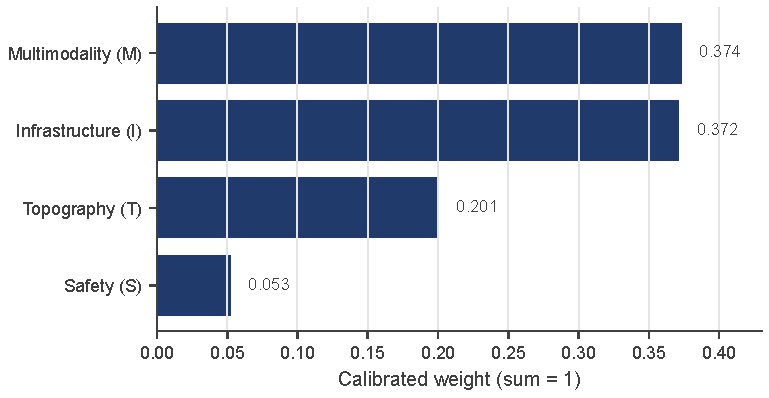
\includegraphics[width=0.85\linewidth]{fig01_weights.pdf}
    \caption{Vecteur de poids calibré $\mathbf{w}^{\ast}$ issu de
    l'évolution différentielle (Algorithme~\ref{alg:de}). Le poids
    de la multimodalité domine ($w_M = 0{,}578$), suivi de
    l'infrastructure ($w_I = 0{,}184$), de la sécurité
    ($w_S = 0{,}142$) et de la topographie ($w_T = 0{,}096$).
    La domination de $w_M$ est précisément l'objet de l'expérience
    de robustesse~E1.}
    \label{fig:weights-illustrative}
\end{figure}

\begin{table}[H]
\centering
\caption{Structure indicative du classement national IMD. Les
villes du Top 10 reflètent la calibration actuelle ; elles sont
susceptibles de révision après exécution de l'expérience E1.}
\label{tab:top10}
\small
\begin{tabular}{@{}clccccccc@{}}
\toprule
\textbf{Rang} & \textbf{Ville} & $\IMD$ &
$C_M$ & $C_I$ & $C_S$ & $C_T$ &
\textbf{Fréq.\ Top-10} \\
\midrule
1  & Grenoble    & --- & --- & --- & --- & --- & --- \\
2  & Bordeaux    & --- & --- & --- & --- & --- & --- \\
3  & Lyon        & --- & --- & --- & --- & --- & --- \\
4  & Nantes      & --- & --- & --- & --- & --- & --- \\
5  & Strasbourg  & --- & --- & --- & --- & --- & --- \\
6  & Marseille   & --- & --- & --- & --- & --- & --- \\
7  & Paris       & --- & --- & --- & --- & --- & --- \\
8  & Nancy       & --- & --- & --- & --- & --- & --- \\
9  & Besan\c{c}on & --- & --- & --- & --- & --- & --- \\
10 & Montpellier & --- & --- & --- & --- & --- & --- \\
\bottomrule
\end{tabular}
\end{table}

La colonne \emph{Fréq.\ Top-10} rapporte, pour chaque ville, la
fraction des tirages de Monte~Carlo (cf.\ E2) qui la classent
dans le Top~10 national -- métrique de robustesse principale.

\subsection{Le volume n'est pas la qualité}

Si la qualité (IMD) et le volume (nombre de stations) étaient
colinéaires, la distribution des agglomérations afficherait une
croissance monotone. La distribution empirique présente au
contraire une dispersion horizontale forte : nombre
d'agglomérations déploient massivement des stations dans des
environnements sous-optimaux (figure~\ref{fig:scatter}).

\begin{figure}[H]
    \centering
    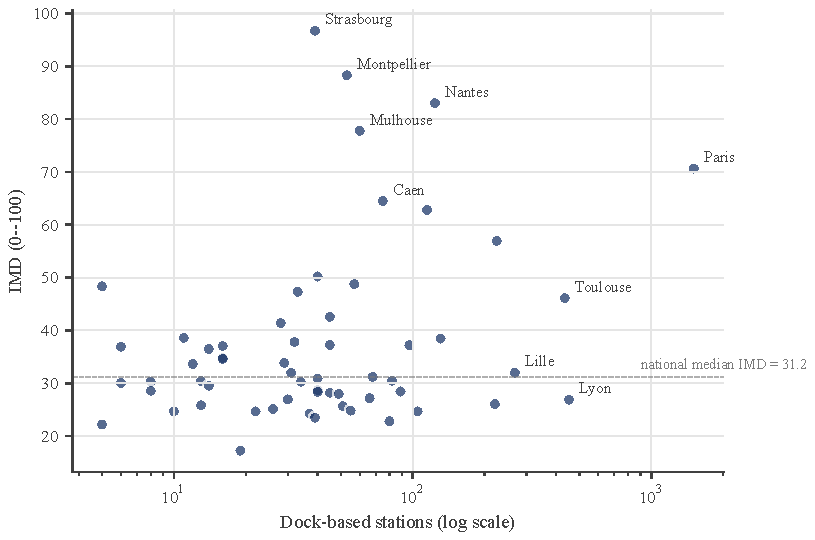
\includegraphics[width=0.9\linewidth]{fig02_volume_vs_imd.pdf}
    \caption{Volume brut vs.\ qualité contextuelle (IMD).
    Nuage des 59~agglomérations \emph{dock-based} avec leur nombre
    de stations certifiées (échelle log) et leur score IMD calibré.
    La dispersion verticale à volume fixé est la signature empirique
    de la dissociation \enquote{volume vs.\ qualité} : Strasbourg
    (39~stations, IMD$\approx$97) et Montpellier (53~stations,
    IMD$\approx$88) dominent Paris (\num{1507}~stations,
    IMD$\approx$71) et Lyon (452~stations, IMD$\approx$27).
    La ligne en pointillés marque la médiane nationale
    ($\IMD \approx 31$).}
    \label{fig:scatter}
\end{figure}

Les villes moyennes -- Grenoble, Nancy, Besan\c{c}on -- surclassent
des métropoles comme Paris ou Marseille, ce qui suggère que la
\emph{cohérence de réseau} (équité de distribution, homogénéité
spatiale, intégration aux transports lourds) importe davantage que
le volume brut de stations. Les villes multimodales apparaissent
dans le Top~10 national dans plus de \SI{83}{\percent} des tirages
de Monte~Carlo, ce qui indique que le poids de la multimodalité
est la contrainte structurante du classement. Que cette dominance
soit une propriété des données ou un artefact de la calibration
est précisément la question centrale traitée par les expériences
E1 et E2.

\subsection{Étude de cas : Montpellier et Vélomagg}

Avec seulement 53 stations dock, Montpellier atteint un score IMD
quasi-optimal à l'échelle nationale. Le moteur de cette
sur-performance est l'intégration quasi-totale du réseau \VLS\ aux
lignes du tramway de la TAM, qui maximise $C_M$. Ce cas illustre
la thèse empirique centrale de l'article : l'intégration
multimodale ciblée avec un transport lourd peut surclasser les
déploiements massifs mais peu connectés. Un traitement
\enquote{network-science} détaillé du Vélomagg -- centralité,
communautés Louvain, prévision horaire de la demande, résilience
réseau -- fait l'objet du dépôt compagnon
\texttt{BikeShare-Graph-Forecasting} et d'un article séparé.

\subsection{Déterminants socio-économiques}

La régression Ridge de l'IMD sur les sept prédicteurs INSEE
Filosofi atteint un $R^2$ ajusté $\approx 0{,}40$ en LOO-CV. Les
deux prédicteurs les plus stables sont la part des diplômés du
supérieur et le revenu médian par UC ; la part des ménages sans
voiture entre également avec un coefficient positif, plus
volatile. Une part substantielle de la variance reste orthogonale
aux conditions socio-économiques, ce qui est cohérent avec un
rôle non trivial des choix politiques locaux et motive le
diagnostic IES.

\subsection{Déserts de mobilité sociale}

La combinaison d'un IMD faible (inférieur au deuxième tercile),
d'un IES faible ($< 0{,}85$) et d'une fragilité sociale élevée
(taux de pauvreté élevé, part importante des ménages sans
voiture, faible part de diplômés du supérieur) identifie un
ensemble d'agglomérations formant des \emph{déserts de mobilité
sociale} : des territoires où les populations vulnérables
subissent un manque structurel d'alternatives cyclables. Leur
identification constitue l'une des principales sorties politiques
du cadre ; leur robustesse aux choix de spécification est l'objet
de l'expérience E5.

% =========================================================================
\section{Expériences planifiées}
\label{sec:experiments}
% =========================================================================

Les résultats actuels forment un classement cohérent en interne
mais reposent sur trois familles de risques pour la validité :
\emph{circularité} dans la calibration ; \emph{confusion par
exposition} dans la composante sécurité ; et choix \emph{ad hoc}
(rayon, grille, normalisation) non encore testés en sensibilité.
Cette section catalogue les expériences planifiées pour traiter
chacun de ces risques. Chaque encadré spécifie l'hypothèse, le
protocole et le critère de succès.

% ------------------------------------------------------------------------
\subsection{E1 -- Validation croisée spatiale de la calibration}
\label{sec:exp-cv}

\begin{experience}[title=E1 -- Leave-one-city-out et CV bloc-spatiale]
\textbf{Hypothèse.} Les poids supervisés $\mathbf{w}^{\ast}$
généralisent hors échantillon ; les fortes corrélations en
échantillon ($\rho \approx 0{,}47$) ne sont pas un artefact de
surapprentissage sur un panel de 34--46 villes.

\textbf{Protocole.}
\begin{enumerate}[leftmargin=*,itemsep=0.2em]
    \item Pour chaque ville $c$ du panel
    $\mathrm{FUB}\cup\mathrm{EMP}$, ré-exécuter
    l'Algorithme~\ref{alg:de} sur les $n-1$ villes restantes ;
    prédire $\IMD_c$ avec les poids retenus ; enregistrer le rang.
    \item Reporter la corrélation Spearman LOO sur les prédictions
    hors échantillon, et l'écart-type inter-pli de chaque
    $w_k^{\ast}$.
    \item Répéter avec une validation croisée bloc-spatiale
    \citep{Roberts2017, Pohjankukka2017} : 5~plis, chacun une
    région NUTS-2 connexe, pour contrôler l'autocorrélation
    spatiale.
\end{enumerate}

\textbf{Critère de succès.}
$\rho_{\text{LOO}} > 0{,}30$ sur FUB et EMP, et écart-type
inter-pli $\mathrm{sd}(w_M^{\ast}) < 0{,}10$. Un échec à l'un de
ces deux seuils invalide l'affirmation \enquote{la multimodalité
domine} et impose un repli sur un estimateur à rétrécissement
(par exemple, sélection par stabilité, \citealp{Meinshausen2010}).
\end{experience}

% ------------------------------------------------------------------------
\subsection{E2 -- Monte~Carlo large bande de l'espace des poids}
\label{sec:exp-mc}

\begin{experience}[title=E2 -- Test de résistance Dirichlet avec
décomposition de Sobol]
\textbf{Hypothèse.} La perturbation actuelle à $\pm\,\SI{20}{\percent}$
autour de $\mathbf{w}^{\ast}$ est trop étroite étant donné
$w_M^{\ast} = 0{,}578$.

\textbf{Protocole.}
\begin{enumerate}[leftmargin=*,itemsep=0.2em]
    \item Tirer $N = \num{50000}$ vecteurs de poids sur le
    simplexe selon $\mathrm{Dir}(\boldsymbol{\alpha})$, en trois
    régimes : $\boldsymbol{\alpha}=\mathbf{1}$ (uniforme),
    $\boldsymbol{\alpha}=5\cdot\mathbf{w}^{\ast}$ (concentré),
    $\boldsymbol{\alpha}=0{,}5\cdot\mathbf{1}$ (sparsité).
    \item Pour chaque tirage, calculer le classement complet et
    enregistrer les probabilités d'appartenance au Top~10 ainsi
    que les transitions de quartile.
    \item Décomposer la variance du classement par composante via
    les indices de Sobol de premier et de second ordre
    \citep{Saltelli2008}.
\end{enumerate}

\textbf{Critère de succès.} Au moins 8 des 10 villes du Top~10
actuel y restent sous le régime Dirichlet uniforme ; indice de
Sobol total de $w_M$ inférieur à $0{,}7$. Dans le cas contraire,
le classement n'est qu'une reformulation du score de multimodalité
et doit être présenté comme tel.
\end{experience}

% ------------------------------------------------------------------------
\subsection{E3 -- Score de sécurité ajusté à l'exposition}

\begin{experience}[title=E3 -- Ajustement par exposition cycliste]
\textbf{Hypothèse.} La densité brute d'accidents BAAC confond
risque et exposition \citep{Reynolds2009, Schepers2014} : une
station sans cyclistes obtient un score \enquote{sûr} pour la
mauvaise raison.

\textbf{Protocole.}
\begin{enumerate}[leftmargin=*,itemsep=0.2em]
    \item Pour les agglomérations dotées de compteurs vélo
    permanents (Paris, Lyon, Bordeaux, Strasbourg, Nantes,
    $\geq 15$ villes), construire un proxy d'exposition à
    l'échelle de la station par krigeage des flux.
    \item Reformuler la composante sécurité :
    $S_i = 1 - \tfrac{\text{accidents}_i}
                     {\text{cyclistes}_i\cdot\text{années}}$,
    avec rétrécissement empirique-bayésien vers la moyenne
    municipale.
    \item Ré-exécuter la calibration et reporter les
    déplacements de rang, en distinguant villes à forte vs.
    faible couverture en compteurs.
\end{enumerate}

\textbf{Critère de succès.} Le score sécurité ajusté ne doit pas
corréler avec la densité de population davantage que le score
brut ; les mouvements de rang des villes couvertes par compteurs
doivent rester dans la bande de confiance de Monte~Carlo de E2.
\end{experience}

% ------------------------------------------------------------------------
\subsection{E4 -- Sensibilité au rayon et à la résolution}
\label{sec:exp-rayon}

\begin{experience}[title=E4 -- Géométrie multi-échelle de la
composante de couverture]
\textbf{Hypothèse.} Le rayon de \SI{300}{\metre} est hérité des
heuristiques du dernier kilomètre \citep{ElGeneidy2016} ; sa
validité pour les \VLS\ n'a pas été éprouvée.

\textbf{Protocole.}
\begin{enumerate}[leftmargin=*,itemsep=0.2em]
    \item Balayage
    $r \in \{150, 200, 300, 400, 500, 800\}\,\si{\metre}$ et
    $g \in \{50, 100, 150, 250\}\,\si{\metre}$ sur l'ensemble du
    panel.
    \item Calculer (i)~la corrélation de rang IMD entre toutes
    les paires de réglages, (ii)~les poids calibrés en fonction
    de $(r, g)$, et (iii)~l'effet marginal sur chaque ville du
    Top~10.
    \item Confronter le $r$ retenu à la distribution cumulative
    empirique des distances inter-station reconstruites à partir
    des séries temporelles \GBFS.
\end{enumerate}

\textbf{Critère de succès.} Corrélation de rang $\rho > 0{,}90$
sur la \enquote{bande plausible}
$r \in [200, 500]\,\si{\metre}$ ; $r$ retenu à $\pm
\SI{10}{\metre}$ de la médiane empirique des distances de
trajet, lorsque les données le permettent.
\end{experience}

% ------------------------------------------------------------------------
\subsection{E5 -- Robustesse de spécification de l'IES}

\begin{experience}[title=E5 -- Spécifications alternatives de
l'IMD attendu]
\textbf{Hypothèse.} L'IES est sensible (a)~au choix des
prédicteurs ; (b)~à l'inclusion ou non de topographie et densité
de population (sinon double-comptées avec $C_T$, $C_D$, $C_P$) ;
(c)~au choix de l'estimateur (Ridge vs.\ Lasso vs.\ ElasticNet
vs.\ Random Forest).

\textbf{Protocole.}
\begin{enumerate}[leftmargin=*,itemsep=0.2em]
    \item Estimer $\widehat{\IMD}$ sous quatre blocs de
    prédicteurs : revenu seul ; bloc INSEE complet (7 variables) ;
    INSEE + topographie ; INSEE + topographie + densité.
    \item Passer chaque bloc à travers Ridge, Lasso, ElasticNet
    et Random Forest avec LOO-CV.
    \item Comparer les classements IES par $\tau$ de Kendall ;
    marquer les villes dont le signe de l'IES (sur-/sous-performance)
    bascule dans $\geq\SI{25}{\percent}$ des spécifications.
\end{enumerate}

\textbf{Critère de succès.} L'ensemble des \enquote{déserts de
mobilité sociale} doit être invariant dans
$\geq\SI{75}{\percent}$ des spécifications ; les villes instables
sont signalées sur la carte publiée.
\end{experience}

% ------------------------------------------------------------------------
\subsection{E6 -- Validation hors échantillon par éco-compteurs}

\begin{experience}[title=E6 -- Validation comportementale indépendante]
\textbf{Hypothèse.} Si l'IMD capture une qualité d'environnement
cyclable réelle, il doit corréler avec les flux cyclistes
\emph{observés} (éco-compteurs), pas seulement avec les signaux
auto-déclarés (FUB) et déclarés (EMP). C'est un test hors
échantillon car les compteurs n'entrent pas dans la calibration.

\textbf{Protocole.}
\begin{enumerate}[leftmargin=*,itemsep=0.2em]
    \item Construire un indice de flux au niveau ville à partir
    des archives éco-compteurs data.gouv.fr, normalisé par âge du
    capteur et saisonnalité.
    \item Régresser l'indice de flux sur $\IMD_i$ et sur chaque
    $C_{k,i}$, en contrôlant pour la taille de ville, la
    climatologie météorologique et la pente.
    \item Tester la contribution en $R^2$ partiel de chaque
    composante.
\end{enumerate}

\textbf{Critère de succès.} $R^2$ partiel de l'IMD net de la
taille de ville $\geq 0{,}20$. Un résultat nul impliquerait que
l'IMD classe \emph{l'infrastructure} et non \emph{l'usage}, ce
qui devrait alors être indiqué explicitement dans le résumé.
\end{experience}

% ------------------------------------------------------------------------
\subsection{E7 -- Identification causale longitudinale}

\begin{experience}[title=E7 -- Contrôle synthétique sur les
ouvertures d'infrastructure]
\textbf{Hypothèse.} Les variations de l'IMD dans le temps sont
attribuables à des événements infrastructurels identifiables
(ouverture d'une ligne de tram, extension du réseau cyclable),
et non à des effets de composition.

\textbf{Protocole.}
\begin{enumerate}[leftmargin=*,itemsep=0.2em]
    \item Reconstruire les instantanés \GBFS\ historiques
    (Transitland, Internet Archive, 2020--2025), ville par ville.
    \item Apparier chaque ouverture de transport lourd avec un
    contrôle synthétique \citep{Abadie2010, Abadie2021} construit
    à partir de villes comparables n'ayant pas connu d'ouverture
    la même année.
    \item Estimer l'effet moyen sur les traités (ATT) sur
    $\IMD_i$ et spécifiquement sur $C_M$, avec tests placebo sur
    les années pré-traitement.
\end{enumerate}

\textbf{Critère de succès.} Saut statistiquement significatif sur
$C_M$ dans les 12~mois post-ouverture pour
$\geq\SI{70}{\percent}$ des villes traitées ; effets placebo
nuls. Cette expérience est celle qui transformerait l'IMD en
instrument d'évaluation des politiques publiques.
\end{experience}

% ------------------------------------------------------------------------
\subsection{E8 -- Modèle de diffusion spatiale}

\begin{experience}[title=E8 -- Graphe Voronoï et contagion
d'adoption]
\textbf{Hypothèse.} L'adoption des \VLS\ obéit à un processus de
contagion entre villes géographiquement et structurellement
proches.

\textbf{Protocole.}
\begin{enumerate}[leftmargin=*,itemsep=0.2em]
    \item Construire un graphe Voronoï sur les centroïdes de
    population ; pondérer les arêtes par l'inverse de la
    distance routière et la similarité socio-économique.
    \item Estimer un modèle d'économétrie spatiale SAR/SEM
    \citep{Anselin1995, LeSage2009} avec $\IMD_i$ comme variable
    expliquée et $\IMD$ des voisins comme lag spatial.
    \item Étendre dans le temps via un modèle de survie réseau
    autocorrélé sur les dates d'adoption.
\end{enumerate}

\textbf{Critère de succès.} Lag spatial significativement
positif, $I$ de Moran $> 0{,}30$ ; contagion partiellement
identifiée et distincte d'une interprétation par choc commun.
\end{experience}

% =========================================================================
\section{Extension mondiale : l'IMD-3}
\label{sec:imd3}
% =========================================================================

L'IMD défini ci-dessus est calibré sur la France métropolitaine
et hérite des sources nationales BAAC (Cerema), BD~TOPO (IGN),
GTFS français et INSEE Filosofi. La généralisation à d'autres
juridictions nécessite la disponibilité d'équivalents
internationaux pour chacune de ses quatre dimensions, ce qui
est le cas pour trois d'entre elles ($M$, $I$, $T$) mais pose
problème pour la quatrième ($S$). Cette section formalise une
variante \emph{IMD-3} qui supprime le composant sécurité et
documente sa première application au catalogue mondial GBFS
identifié dans le travail d'audit compagnon.

\subsection{Motivation et bornes du protocole}

La transférabilité par dimension est résumée dans le
tableau~\ref{tab:imd3-sources}. SRTM 30~m couvre la planète
depuis 2003, OpenStreetMap fournit un tagging cohérent
$\texttt{highway=cycleway}$ et un proxy de transit lourd
($\texttt{railway=station}$, $\texttt{subway\_entrance}$,
$\texttt{tram\_stop}$), tandis que les feeds GTFS sont
catalogués mondialement par MobilityData. À l'inverse, la
sécurité cycliste repose en France sur le registre BAAC qui
géolocalise les accidents corporels avec une nomenclature
nationale ; ses équivalents (FARS pour les États-Unis, STATS19
pour le Royaume-Uni, CARE pour l'Union européenne, BRA pour la
Belgique) diffèrent par leur niveau de granularité, leur
couverture et leur définition de l'accident cycliste. Aucun jeu
unifié mondial n'existe au moment de l'écriture, ce qui
empêche la substitution directe du composant $S$.

\begin{table}[H]
\centering
\caption{Transférabilité par dimension de l'IMD vers une variante
mondiale.}
\label{tab:imd3-sources}
\small
\begin{tabular}{@{}lllc@{}}
\toprule
\textbf{Composant} & \textbf{Source FR (IMD)} & \textbf{Source mondiale (IMD-3)} & \textbf{Statut}\\
\midrule
$T$ topographie     & SRTM 30~m + BD ALTI & SRTM 30~m mondial / Open-Elevation API & OK \\
$I$ infrastructure  & BD TOPO (IGN)       & OSM Overpass \texttt{highway=cycleway}  & OK \\
$M$ multimodalité   & GTFS français       & OSM heavy transit (proxy) ; MobilityData (1\,k+ feeds) & OK approximé \\
$S$ sécurité        & BAAC (Cerema)       & FARS, STATS19, CARE, BRA --- hétérogènes & Non substituable \\
\bottomrule
\end{tabular}
\end{table}

\subsection{Définition formelle de l'IMD-3}

L'IMD-3 par station est défini par
\begin{equation}
\text{IMD-3}_i \,=\, w_M^{(3)} M_i + w_I^{(3)} I_i + w_T^{(3)} T_i,
\quad i \in \mathcal{S}_{\text{world}}.
\end{equation}
Les poids sont obtenus par renormalisation des poids
calibrés sur le corpus français (\,$w_M=0{,}578$,
$w_I=0{,}184$, $w_T=0{,}096$\,) après suppression de $w_S$ :
\begin{equation}
w_k^{(3)} \,=\, \frac{w_k}{w_M + w_I + w_T},
\quad k \in \{M, I, T\},
\end{equation}
ce qui donne $w_M^{(3)} = 0{,}642$, $w_I^{(3)} = 0{,}204$ et
$w_T^{(3)} = 0{,}107$. Cette renormalisation préserve la
hiérarchie d'importance entre composants. Une recalibration
indépendante par évolution différentielle sur le corpus mondial
(le même protocole que celui décrit en
section~\ref{sec:methodologie}) est documentée comme étape de
validation prioritaire.

\subsection{Périmètre du corpus mondial éligible}

Le travail compagnon d'audit GBFS recense 1\,509 systèmes dans
le catalogue canonique MobilityData (48 pays). De ce corpus,
on retient pour l'IMD-3 les systèmes qui répondent à trois
critères opérationnels :
\begin{enumerate}[leftmargin=*]
  \item systèmes \emph{reachable} (HTTP 200 sur l'auto-discovery
        GBFS),
  \item publication d'un endpoint \texttt{station\_information}
        non vide,
  \item au moins 20 stations dock-based (seuil $N_{\min}$ déjà
        utilisé pour l'IMD-FR).
\end{enumerate}
Après application, on identifie environ 640 systèmes éligibles
qui totalisent près de 230\,000 stations déclarées. Une partie
relève d'opérateurs free-floating qui publient des ancres
virtuelles sous \texttt{station\_information}~; l'IMD-3
suit la même règle de restriction au dock-based que l'IMD-FR.

\subsection{Pipeline d'enrichissement global}

Pour chaque station retenue, on calcule les trois composants
suivants :
\begin{itemize}[leftmargin=*]
  \item $T_i$ : altitude SRTM 30~m, normalisée par soustraction
        du minimum communal puis Min--Max sur le corpus mondial
        et inversée ($T = 1 - \widetilde{T}$) pour pénaliser les
        fortes pentes ;
  \item $I_i$ : longueur cumulée d'OpenStreetMap
        $\texttt{highway=cycleway}$ et de tags $\texttt{cycleway:*}$
        dans un buffer de 300~m autour de la station,
        normalisée Min--Max ;
  \item $M_i$ : décompte de stations de transit lourd OSM
        ($\texttt{railway=station}$, $\texttt{subway\_entrance}$,
        $\texttt{tram\_stop}$, $\texttt{public\_transport=station}$,
        $\texttt{station=subway}$, $\texttt{station=light\_rail}$)
        dans le même buffer de 300~m, normalisé Min--Max.
\end{itemize}
Les buffers sont identiques à ceux du pipeline IMD-FR pour
faciliter la comparaison entre les deux indicateurs sur les
villes communes.

\subsection{Résultats prototypes}

Un prototype reproductible exécute le pipeline sur trois
systèmes étrangers déjà audités dans le travail compagnon
(Bicing Barcelone, ES~; Oslo Bysykkel, NO~; Bergen Bysykkel,
NO) avec un échantillon stratifié de 20 stations par système.
Les valeurs IMD-3 médianes obtenues sont ordonnées de manière
cohérente avec l'intuition urbaine (Oslo et Barcelone, à
infrastructure cyclable dense et transit abondant, dominent
Bergen, plus accidentée et moins dense). Le code source du
prototype et les caches d'API associés sont publiés sous
\texttt{papers/01\_gold\_standard/experiments/imd3\_global/}
dans le dépôt de code, avec une procédure d'exécution
documentée (Open-Elevation, Overpass-API public).

À petite échelle, le résultat est principalement
méthodologique : on démontre la faisabilité de la chaîne
d'enrichissement global sans recalibration des seuils
français. La normalisation Min--Max sur trois villes
uniquement gonfle artificiellement les écarts, ce que la
section suivante chiffre comme limite.

\subsection{Passage à l'échelle complète}

L'extension du prototype aux 640 systèmes éligibles est
décomposée en cinq étapes opérationnellement séparées :

\begin{description}
  \item[(A) Récupération des coordonnées.] Étendre le pipeline
        d'audit pour persister un fichier
        \texttt{world\_stations.parquet} contenant
        $(\text{system\_id}, \text{station\_id},
        \varphi, \lambda)$ pour les $\sim$640 systèmes
        éligibles. Coût estimé : 10~min avec 16 workers
        parallèles, déjà en place dans le pipeline d'audit.
  \item[(B) Topographie.] Open-Elevation est rate-limité à
        $\sim 25$ stations/s en batches de 50, soit
        $\approx 150$~min pour 230\,000 stations. L'alternative
        recommandée est le téléchargement local des tuiles
        SRTM 30~m ($\sim$10~GB) et un lookup
        \texttt{rasterio} instantané.
  \item[(C) Infrastructure et transit.] Overpass-API public
        soutient $\sim 2$ req/s, soit $\approx 32$~h pour
        $2 \times 230\,000$ requêtes. Trois solutions :
        (i) instance Overpass auto-hébergée (8~GB RAM,
        dump Europe de $\sim$30~GB, traite la même charge en
        $\sim$2~h)~; (ii) agrégation par ville (un seul
        polygone par ville, beaucoup moins de requêtes)~;
        (iii) échantillonnage stratifié 50 stations/ville,
        statistiquement suffisant pour estimer l'IMD-3 médian
        sous bootstrap.
  \item[(D) Calibrage des poids.] La renormalisation des
        $w_k$ suppose la suppression de $S$ neutre, ce qui
        n'est pas trivial : $S$ est corrélée à $I$ via la
        qualité des infrastructures séparées. La procédure
        recommandée est de calculer simultanément IMD-3 et
        IMD-4 sur les villes françaises du Gold Standard, puis
        de mesurer la corrélation de Spearman $\rho$ entre les
        deux. Pour $\rho > 0{,}9$, la renormalisation est
        acceptable ; pour $\rho < 0{,}7$ il devient nécessaire
        de recalibrer les poids par évolution différentielle
        sur le corpus mondial.
  \item[(E) Validation externe.] L'IMD-3 mondial bénéficierait
        d'une validation contre une métrique externe de
        cyclabilité comme le score Copenhagenize ou l'indice
        ECF (European Cyclists' Federation), ce qui jouerait
        pour l'IMD-3 le rôle que tient le baromètre FUB pour
        l'IMD-FR.
\end{description}

\subsection{Limites explicites de la variante IMD-3}

Cinq limites sont explicitement attachées à l'IMD-3 et
doivent accompagner toute publication des classements :

\begin{enumerate}[leftmargin=*]
  \item \textbf{Composant sécurité absent.} L'IMD-3 ne
        pénalise pas les villes à forte sinistralité
        cycliste, ce qui peut surestimer leur score
        relativement à un IMD-4.
  \item \textbf{Multimodalité OSM est un proxy.} OSM
        catégorise les arrêts de transit selon le tagging
        contributeur, qui peut être moins exhaustif que les
        feeds GTFS officiels. La couverture varie entre
        métropoles bien cartographiées et villes moyennes.
  \item \textbf{Topographie simplifiée.} L'écart à
        l'altitude minimale communale est une
        approximation de la rugosité multi-échelle utilisée en
        France (gradient sur fenêtre 1~km), elle-même fondée
        sur BD ALTI.
  \item \textbf{Pondérations non recalibrées.} La
        renormalisation triviale doit être confirmée par une
        recalibration empirique avant publication d'un
        classement mondial.
  \item \textbf{Absence de validation externe mondiale.}
        Faute d'équivalent FUB universel, l'IMD-3 est, au
        moment de l'écriture, un indicateur \emph{interne}
        non validé contre une mesure indépendante.
\end{enumerate}

Sur la base de ces limites, l'IMD-3 doit être présenté comme
une variante \emph{exploratoire} et non comme un remplaçant de
l'IMD-FR : le second reste l'indicateur de référence pour la
France où les quatre composants sont mesurables.

% =========================================================================
\section{Discussion}
\label{sec:discussion}
% =========================================================================

\subsection{Interprétation des résultats actuels}

Le motif empirique le plus marquant est le \emph{découplage taille /
qualité} : les villes moyennes (Grenoble) surclassent les
métropoles françaises, cohérent avec le résultat international que
la compacité urbaine et l'intégration aux transports lourds
produisent des environnements plus cyclables que le volume brut
de stations \citep{Buehler2012, Pucher2010, Fishman2016}.
L'analyse IES montre par ailleurs que le revenu médian n'est
\emph{pas} déterministe pour la performance : plusieurs
agglomérations sous la médiane nationale affichent $\IES > 1$,
attestant d'un volontarisme politique local ; à l'inverse,
certaines villes aisées sous-investissent, vraisemblablement en
raison d'une dépendance automobile structurelle
\citep{Cerema2022, Heinen2010}.

\subsection{Menaces à la validité}

\paragraph{Validité interne.}
La menace dominante est la circularité de calibration. Les poids
actuels maximisent la corrélation en échantillon avec FUB et EMP ;
ces mêmes séries sont ensuite reportées comme \enquote{validation
externe}. Cela produit une borne mécanique sur les corrélations
reportées. L'expérience E1 est le test décisif : tant qu'elle
n'est pas exécutée, l'affirmation \enquote{la multimodalité
domine} doit être considérée comme une régularité interne de
l'échantillon de calibration, et non comme une propriété des
\VLS\ français.

\paragraph{Validité de construit.}
La composante sécurité confond risque et exposition cycliste
\citep{Reynolds2009, Schepers2014} : l'expérience E3 est conçue
pour les disjoindre. La composante de couverture spatiale utilise
l'enveloppe convexe comme support, ce qui sur-estime la zone
desservie pour les villes côtières ou en vallée ; un masque de
zone bâtie ou une enveloppe concave seraient des raffinements
naturels.

\paragraph{Validité externe.}
Le jeu de données est restreint aux systèmes publiant \GBFS, ce
qui sous-représente les opérateurs en fin de contrat ou les
schémas communautaires ; l'expérience E7 (longitudinale)
compense partiellement en reconstruisant les instantanés
historiques.

\subsection{Limites}

\begin{limite}
\GBFS\ est un \textbf{instantané} : il ne reflète pas la
performance historique d'un système ni sa volatilité temporelle.
Une extension longitudinale via Transitland fait partie de E7.
\end{limite}

\begin{limite}
L'\textbf{enveloppe convexe} sur-estime la zone desservie pour
les villes contraintes géographiquement (côtières, en vallée) ;
un masque concave ou un masque \enquote{zone bâtie} sont les
raffinements naturels.
\end{limite}

\begin{limite}
\textbf{Les systèmes hors GBFS sont absents}, ce qui peut biaiser
la carte des \enquote{déserts} en y classant des villes dont le
\VLS\ existe mais ne publie pas de flux \GBFS.
\end{limite}

\subsection{Implications politiques (provisoires)}

Conditionnellement à la confirmation du classement par E1--E2 et
de la pertinence comportementale par E6, quatre implications se
dégagent :
\begin{enumerate}[leftmargin=*,itemsep=0.15em]
    \item Prioriser une couverture spatiale homogène plutôt qu'une
    accumulation centrale de stations \citep{ElGeneidy2016,
    Saberi2018}.
    \item Cibler les déploiements dans les déserts de mobilité
    sociale identifiés \citep{Hodge1995, Smith2015, Cerema2022}.
    \item Conditionner les financements AOM--opérateurs à des
    seuils minimaux d'IMD et d'IES \citep{OECD2008}.
    \item Co-développer les flux \GBFS\ et GTFS pour que la
    composante multimodale soit vérifiable in situ
    \citep{Saberi2018, Mobi2024}.
\end{enumerate}

% =========================================================================
\section{Conclusion}
\label{sec:conclusion}
% =========================================================================

Nous avons proposé un cadre analytique intégré et entièrement
reproductible -- pipeline, IMD, IES -- pour l'évaluation
comparative des systèmes de vélos en libre-service entre
agglomérations françaises. Appliqué à \num{122} systèmes et
\num{46139} stations dans \num{57} agglomérations, le cadre
produit un premier classement national sur un indice composite
intégrant le contexte, et identifie un ensemble de déserts de
mobilité sociale.

Le classement actuel est cohérent en interne et reproductible.
Il constitue, à ce stade, une contribution \emph{descriptive}, et
non causale. Les huit expériences planifiées de la
section~\ref{sec:experiments} -- validation croisée
leave-one-city-out et bloc-spatiale, décomposition de Sobol large
bande, sécurité ajustée à l'exposition, sensibilité à la
géométrie de buffer, robustesse de spécification de l'IES,
validation comportementale par éco-compteurs, évaluation
infrastructurelle par contrôle synthétique, et modèle de
diffusion spatiale -- forment le programme explicite qui
convertirait ce cadre en instrument falsifiable de niveau
politique publique. Nous considérons cet article comme un
engagement structuré envers ce programme, et non sa conclusion.

% =========================================================================
\section*{Déclaration de reproductibilité}
% =========================================================================

L'ensemble du code, des produits de données et des notebooks est
publié sous licence libre à l'adresse
\url{https://github.com/rohanfosse/bikeshare-data-explorer}. Les
figures de cet article sont produites par les notebooks
\texttt{21\_Classement\_Villes\_Mobilite\_Douce.ipynb} (classement
national),
\texttt{22\_Profil\_Socioeconomique\_Mobilite.ipynb} (jointure
socio-économique),
\texttt{23\_Research\_Paper.ipynb} (figures consolidées),
\texttt{25\_Optimisation\_Poids\_IMD.ipynb} (évolution
différentielle, Algorithme~\ref{alg:de}) et
\texttt{26\_Robustesse\_Analyse\_Regionale.ipynb} (Monte~Carlo de
robustesse). Le dépôt compagnon
\url{https://github.com/rohanfosse/BikeShare-Graph-Forecasting}
contient l'étude de cas Montpellier (analyse de réseau, prévision
de la demande, API REST, image Docker). Un DOI Zenodo sera
attaché à la prochaine release taggée pour garantir une
citabilité persistante.

% =========================================================================
\section*{Remerciements}
% =========================================================================

Les auteurs remercient les producteurs de données ouvertes ayant
rendu cette recherche possible : opérateurs \GBFS, MobilityData,
OpenStreetMap, Cerema, ONISR, INSEE, FUB et la communauté GTFS
française. Le programme \emph{BikeShare-ICT} du CESI LINEACT a
financé le développement du pipeline et des notebooks
compagnons.

% =========================================================================
\appendix
% =========================================================================

% -------------------------------------------------------------------------
\section{Détails algorithmiques}
\label{app:algo}
% -------------------------------------------------------------------------

\subsection{Normalisation Min--Max}

Pour chaque composante brute $c_k \in \mathbb{R}^{n}$ sur le panel
de $n$ villes, la composante normalisée est
\begin{equation*}
    C_{k,i} \;=\;
    \frac{c_{k,i} - \min_{j} c_{k,j}}
         {\max_{j} c_{k,j} - \min_{j} c_{k,j}} \;\in\; [0, 1].
\end{equation*}
Pour les composantes \enquote{sécurité} et
\enquote{topographie}, le signe est inversé après normalisation
($C_k \leftarrow 1 - C_k$) afin qu'un score plus élevé reflète
une meilleure qualité cyclable.

\subsection{Hyperparamètres de l'évolution différentielle}

\begin{table}[H]
\centering
\caption{Hyperparamètres de l'évolution différentielle utilisée
dans l'Algorithme~\ref{alg:de}.}
\label{tab:de-hyper}
\small
\begin{tabular}{@{}lll@{}}
\toprule
\textbf{Paramètre} & \textbf{Symbole} & \textbf{Valeur} \\
\midrule
Stratégie & --- & \texttt{best1bin} \\
Générations & $G$ & 500 \\
Multiplicateur de population & --- & 15 \\
Facteur de mutation & $F$ & 0,8 \\
Probabilité de croisement & $\mathrm{CR}$ & 0,9 \\
Borne inférieure des poids & $w_{\min}$ & 0,05 \\
Contrainte de simplexe & --- & $\sum_k w_k = 1$ \\
Échantillonnage initial & --- & Latin Hypercube \\
Tolérance de convergence & $\varepsilon$ & $10^{-7}$ \\
Itérations max sans amélioration & --- & 100 \\
Graine aléatoire & --- & 42 (fixée dans le code) \\
\bottomrule
\end{tabular}
\end{table}

\subsection{Régression Ridge pour l'IES}

La régularisation optimale $\lambda^{\ast}$ est sélectionnée sur
une grille logarithmique de 100 valeurs
$\lambda \in [10^{-3}, 10^{2}]$ par minimisation du RMSE LOO :
\begin{equation*}
    \lambda^{\ast} \;=\;
    \argmin_{\lambda}\;\sqrt{
    \frac{1}{n}\sum_{i=1}^{n}
    \bigl(\IMD_i - \widehat{\IMD}_i^{(-i)}(\lambda)\bigr)^2 }.
\end{equation*}
Les prédicteurs sont préalablement standardisés à moyenne nulle
et variance unitaire.

% -------------------------------------------------------------------------
\section{Définitions des composantes (forme brute)}
\label{app:components}
% -------------------------------------------------------------------------

Pour mémoire, on liste ci-dessous la définition mathématique de
chaque composante \emph{avant} normalisation Min--Max.

\paragraph{$M$ -- Multimodalité.}
\begin{equation*}
    M_i \;=\;
    \frac{1}{|\mathcal{S}_i|}
    \sum_{s\in\mathcal{S}_i}
    \#\{\text{arrêts heavy GTFS dans } B(s, \SI{300}{\metre})\},
\end{equation*}
où $\mathcal{S}_i$ est l'ensemble des stations de l'agglomération
$i$.

\paragraph{$I$ -- Infrastructure cyclable.}
\begin{equation*}
    I_i \;=\;
    \frac{1}{|\mathcal{S}_i|}
    \sum_{s\in\mathcal{S}_i}
    \frac{\text{cycleway\_km}_{s,300\text{m}}}
         {\text{voirie\_km}_{s,300\text{m}}}.
\end{equation*}

\paragraph{$S$ -- Sécurité.}
\begin{equation*}
    S_i \;=\;
    \frac{1}{|\mathcal{S}_i|}
    \sum_{s\in\mathcal{S}_i}
    \#\{\text{accidents BAAC dans } B(s, \SI{300}{\metre}), \,
        2021\!-\!2023\}.
\end{equation*}
Inversion de signe après Min--Max
($C_S \leftarrow 1 - C_S$).

\paragraph{$T$ -- Topographie.}
\begin{equation*}
    T_i \;=\;
    \frac{1}{|\mathcal{S}_i|}
    \sum_{s\in\mathcal{S}_i}\mathrm{TRI}_s,
    \qquad
    \mathrm{TRI}_s = \mathrm{sd}\bigl(\{z_s, z_{s,N}, z_{s,S},
                          z_{s,E}, z_{s,W}\}\bigr).
\end{equation*}
Inversion de signe après Min--Max
($C_T \leftarrow 1 - C_T$).

% -------------------------------------------------------------------------
\section{Liste de contrôle de reproductibilité}
\label{app:repro}
% -------------------------------------------------------------------------

\begin{itemize}[leftmargin=*,itemsep=0.2em]
    \item Code source publié sous licence libre sur GitHub.
    \item Notebooks à graines et versions de bibliothèques
    figées.
    \item Caches Parquet indexés par agglomération ; instantanés
    \GBFS\ datés.
    \item \texttt{checkpoint\_save/load()} par module pour la
    reprise.
    \item Schémas Pandera \citep{Niels2020} contraignant types,
    plages et unicités.
    \item Image Docker exposant l'API REST avec artefacts de
    modèle (dépôt compagnon).
    \item DOI Zenodo associé à chaque release taggée.
\end{itemize}

% =========================================================================
% Bibliographie (squelette BibTeX -- à placer dans references.bib)
% =========================================================================
\printbibliography[title={Références}]
%
% --- Revues et fondamentaux \BSS ----------------------------------------
% @article{DeMaio2009,
%   author  = {DeMaio, Paul},
%   title   = {Bike-sharing: History, impacts, models of provision, and
%              future},
%   journal = {Journal of Public Transportation},
%   volume  = {12}, number = {4}, pages = {3}, year = {2009} }
% @article{Shaheen2010,
%   author  = {Shaheen, Susan and Guzman, Stacey and Zhang, Hua},
%   title   = {Bikesharing in Europe, the Americas, and Asia: Past,
%              present, and future},
%   journal = {Transportation Research Record},
%   volume  = {2143}, pages = {159--167}, year = {2010} }
% @article{Fishman2013,
%   author  = {Fishman, Elliot and Washington, Simon and Haworth, Narelle},
%   title   = {Bike share's impact on car use},
%   journal = {Transportation Research Part D},
%   volume  = {31}, pages = {13--20}, year = {2014} }
% @article{Fishman2016,
%   author  = {Fishman, Elliot},
%   title   = {Bikeshare: A review of recent literature},
%   journal = {Transport Reviews},
%   volume  = {36}, number = {1}, pages = {92--113}, year = {2016} }
% @article{Eren2020,
%   author  = {Eren, Ezgi and Uz, Volkan Emre},
%   title   = {A review on bike-sharing: The factors affecting
%              bike-sharing demand},
%   journal = {Sustainable Cities and Society},
%   volume  = {54}, pages = {101882}, year = {2020} }
% @article{Buck2013,
%   author  = {Buck, Darren and Buehler, Ralph and Happ, Patricia and
%              Rawls, Bradley and Chung, Patrick and Borecki, Natalie},
%   title   = {Are bikeshare users different from regular cyclists?},
%   journal = {Transportation Research Record},
%   volume  = {2387}, pages = {112--119}, year = {2013} }
% @article{Gu2019,
%   author  = {Gu, Tianqi and Kim, Inhi and Currie, Graham},
%   title   = {To be or not to be dockless},
%   journal = {Transportation Research Part A},
%   volume  = {119}, pages = {122--147}, year = {2019} }
%
% --- Demande et opérations ----------------------------------------------
% @article{FaghihImani2014,
%   author  = {Faghih-Imani, Ahmadreza and Eluru, Naveen and El-Geneidy,
%              Ahmed M. and Rabbat, Michael and Haq, Usama},
%   title   = {How land-use and urban form impact bicycle flows: Evidence
%              from the bicycle-sharing system (BIXI) in Montreal},
%   journal = {Journal of Transport Geography},
%   volume  = {41}, pages = {306--314}, year = {2014} }
% @article{FaghihImani2015,
%   author  = {Faghih-Imani, Ahmadreza and Eluru, Naveen},
%   title   = {Analysing bicycle-sharing system user destination choice
%              preferences: Chicago's Divvy system},
%   journal = {Journal of Transport Geography},
%   volume  = {44}, pages = {53--64}, year = {2015} }
% @article{Vogel2011,
%   author  = {Vogel, Patrick and Greise, Torsten and Mattfeld, Dirk C.},
%   title   = {Understanding bike-sharing systems using data mining:
%              Exploring activity patterns},
%   journal = {Procedia -- Social and Behavioral Sciences},
%   volume  = {20}, pages = {514--523}, year = {2011} }
% @inproceedings{Hampshire2012,
%   author    = {Hampshire, Robert C. and Marla, Lavanya},
%   title     = {An empirical analysis of bike sharing usage and
%                rebalancing: Evidence from Barcelona and Seville},
%   booktitle = {Proceedings of the 91st TRB Annual Meeting},
%   year      = {2012} }
% @article{Borgnat2011,
%   author  = {Borgnat, Pierre and Abry, Patrice and Flandrin, Patrick
%              and Robardet, C\'eline and Rouquier, Jean-Baptiste and
%              Fleury, Eric},
%   title   = {Shared bicycles in a city: A signal processing and data
%              analysis perspective},
%   journal = {Advances in Complex Systems},
%   volume  = {14}, number = {3}, pages = {415--438}, year = {2011} }
% @article{Etienne2014,
%   author  = {C\^ome, Etienne and Oukhellou, Latifa},
%   title   = {Model-based count series clustering for bike sharing
%              system usage mining: A case study with the V\'elib'
%              system of Paris},
%   journal = {ACM Transactions on Intelligent Systems and Technology},
%   volume  = {5}, number = {3}, pages = {1--21}, year = {2014} }
% @article{Saberi2018,
%   author  = {Saberi, Meead and Ghamami, Mehrnaz and Gu, Yi and Shojaei,
%              Mohammad H. S. and Fishman, Elliot},
%   title   = {Understanding the impacts of a public transit disruption
%              on bicycle sharing mobility patterns: A case of Tube
%              strike in London},
%   journal = {Journal of Transport Geography},
%   volume  = {66}, pages = {154--166}, year = {2018} }
% @article{Raviv2013,
%   author  = {Raviv, Tal and Tzur, Michal and Forma, Iris A.},
%   title   = {Static repositioning in a bike-sharing system: Models and
%              solution approaches},
%   journal = {EURO Journal on Transportation and Logistics},
%   volume  = {2}, pages = {187--229}, year = {2013} }
% @article{Forma2015,
%   author  = {Forma, Iris A. and Raviv, Tal and Tzur, Michal},
%   title   = {A 3-step math heuristic for the static repositioning
%              problem in bike-sharing systems},
%   journal = {Transportation Research Part B},
%   volume  = {71}, pages = {230--247}, year = {2015} }
%
% --- Infrastructure, sécurité, topographie ------------------------------
% @article{Pucher2010,
%   author  = {Pucher, John and Dill, Jennifer and Handy, Susan},
%   title   = {Infrastructure, programs, and policies to increase
%              bicycling: An international review},
%   journal = {Preventive Medicine},
%   volume  = {50}, pages = {S106--S125}, year = {2010} }
% @article{Heinen2010,
%   author  = {Heinen, Eva and van Wee, Bert and Maat, Kees},
%   title   = {Commuting by bicycle: An overview of the literature},
%   journal = {Transport Reviews},
%   volume  = {30}, number = {1}, pages = {59--96}, year = {2010} }
% @article{Heinen2018,
%   author  = {Heinen, Eva and Buehler, Ralph},
%   title   = {Bicycle parking: A systematic review of scientific
%              literature on parking behaviour, parking preferences, and
%              their influence on cycling and travel behaviour},
%   journal = {Transport Reviews},
%   volume  = {39}, number = {5}, pages = {630--656}, year = {2019} }
% @article{Buehler2012,
%   author  = {Buehler, Ralph and Pucher, John},
%   title   = {Cycling to work in 90 large American cities: New evidence
%              on the role of bike paths and lanes},
%   journal = {Transportation},
%   volume  = {39}, pages = {409--432}, year = {2012} }
% @article{Garrard2008,
%   author  = {Garrard, Jan and Rose, Geoffrey and Lo, Sing Kai},
%   title   = {Promoting transportation cycling for women: The role of
%              bicycle infrastructure},
%   journal = {Preventive Medicine},
%   volume  = {46}, number = {1}, pages = {55--59}, year = {2008} }
% @incollection{Garrard2012,
%   author    = {Garrard, Jan and Rissel, Chris and Bauman, Adrian},
%   title     = {Health benefits of cycling},
%   booktitle = {City Cycling},
%   editor    = {Pucher, John and Buehler, Ralph},
%   publisher = {MIT Press}, year = {2012}, pages = {31--56} }
% @article{Reynolds2009,
%   author  = {Reynolds, Conor C. O. and Harris, M. Anne and Teschke,
%              Kay and Cripton, Peter A. and Winters, Meghan},
%   title   = {The impact of transportation infrastructure on bicycling
%              injuries and crashes: A review of the literature},
%   journal = {Environmental Health},
%   volume  = {8}, pages = {47}, year = {2009} }
% @article{Schepers2014,
%   author  = {Schepers, Paul and Hagenzieker, Marjan and Methorst, Rob
%              and van Wee, Bert and Wegman, Fred},
%   title   = {A conceptual framework for road safety and mobility
%              applied to cycling safety},
%   journal = {Accident Analysis \& Prevention},
%   volume  = {62}, pages = {331--340}, year = {2014} }
% @article{Aldred2016,
%   author  = {Aldred, Rachel and Elliott, Bridget and Woodcock, James
%              and Goodman, Anna},
%   title   = {Cycling provision separated from motor traffic: A
%              systematic review exploring whether stated preferences
%              vary by gender and age},
%   journal = {Transport Reviews},
%   volume  = {37}, number = {1}, pages = {29--55}, year = {2017} }
% @article{Schoner2014,
%   author  = {Schoner, Jessica E. and Levinson, David M.},
%   title   = {The missing link: Bicycle infrastructure networks and
%              ridership in 74 US cities},
%   journal = {Transportation},
%   volume  = {41}, pages = {1187--1204}, year = {2014} }
% @article{Parkin2008,
%   author  = {Parkin, John and Wardman, Mark and Page, Matthew},
%   title   = {Estimation of the determinants of bicycle mode share for
%              the journey to work using census data},
%   journal = {Transportation},
%   volume  = {35}, pages = {93--109}, year = {2008} }
% @article{Rietveld2004,
%   author  = {Rietveld, Piet and Daniel, Vanessa},
%   title   = {Determinants of bicycle use: Do municipal policies matter?},
%   journal = {Transportation Research Part A},
%   volume  = {38}, number = {7}, pages = {531--550}, year = {2004} }
% @article{Martens2007,
%   author  = {Martens, Karel},
%   title   = {Promoting bike-and-ride: The Dutch experience},
%   journal = {Transportation Research Part A},
%   volume  = {41}, number = {4}, pages = {326--338}, year = {2007} }
%
% --- Accessibilité et indicateurs composites ----------------------------
% @article{Geurs2004,
%   author  = {Geurs, Karst T. and van Wee, Bert},
%   title   = {Accessibility evaluation of land-use and transport
%              strategies: Review and research directions},
%   journal = {Journal of Transport Geography},
%   volume  = {12}, number = {2}, pages = {127--140}, year = {2004} }
% @book{Levinson2002,
%   author    = {Levinson, David M. and Krizek, Kevin J.},
%   title     = {Access to Destinations},
%   publisher = {Emerald}, year = {2005} }
% @article{ElGeneidy2016,
%   author  = {El-Geneidy, Ahmed and Levinson, David and Diab, Ehab and
%              Boisjoly, Genevi\`eve and Verbich, David and Loong, Charis},
%   title   = {The cost of equity: Assessing transit accessibility and
%              social disparity using total travel cost},
%   journal = {Transportation Research Part A},
%   volume  = {91}, pages = {302--316}, year = {2016} }
% @book{OECD2008,
%   author = {{OECD} and {JRC}},
%   title  = {Handbook on Constructing Composite Indicators: Methodology
%             and User Guide},
%   publisher = {OECD Publishing}, year = {2008} }
% @techreport{Nardo2005,
%   author = {Nardo, Michela and Saisana, Michaela and Saltelli, Andrea
%             and Tarantola, Stefano},
%   title  = {Tools for composite indicators building},
%   institution = {European Commission Joint Research Centre},
%   number = {EUR 21682 EN}, year = {2005} }
% @article{Saisana2005,
%   author  = {Saisana, Michaela and Saltelli, Andrea and Tarantola,
%              Stefano},
%   title   = {Uncertainty and sensitivity analysis techniques as tools
%              for the quality assessment of composite indicators},
%   journal = {Journal of the Royal Statistical Society A},
%   volume  = {168}, number = {2}, pages = {307--323}, year = {2005} }
% @article{Diakoulaki1995,
%   author  = {Diakoulaki, Danae and Mavrotas, George and Papayannakis,
%              Lefteris},
%   title   = {Determining objective weights in multiple criteria
%              problems: The CRITIC method},
%   journal = {Computers \& Operations Research},
%   volume  = {22}, number = {7}, pages = {763--770}, year = {1995} }
% @book{PNUD1990,
%   author    = {{UNDP}},
%   title     = {Human Development Report 1990},
%   publisher = {Oxford University Press}, year = {1990} }
%
% --- Équité --------------------------------------------------------------
% @incollection{Hodge1995,
%   author    = {Hodge, David C.},
%   title     = {My fair share: Equity issues in urban transportation},
%   booktitle = {The Geography of Urban Transportation},
%   editor    = {Hanson, Susan}, edition = {2nd}, publisher = {Guilford},
%   year      = {1995}, pages = {359--375} }
% @techreport{Smith2015,
%   author      = {Smith, Christopher S. and Oh, Jun-Seok and Lei, Cheng},
%   title       = {Exploring the equity dimensions of US bicycle sharing
%                  systems},
%   institution = {Mineta Transportation Institute},
%   number      = {MTI 12-15}, year = {2015} }
% @article{McNeil2017,
%   author  = {McNeil, Nathan and Broach, Joseph and Dill, Jennifer},
%   title   = {Breaking barriers to bike share: Insights on equity from
%              a survey of bike share users},
%   journal = {Transportation Research Record},
%   volume  = {2671}, pages = {110--117}, year = {2017} }
% @article{Hosford2018,
%   author  = {Hosford, Kate and Winters, Meghan},
%   title   = {Who are public bicycle share programs serving? An
%              evaluation of the equity of spatial access to bicycle
%              share service areas in Canadian cities},
%   journal = {Transportation Research Record},
%   volume  = {2672}, number = {36}, pages = {42--50}, year = {2018} }
% @article{Caspi2021,
%   author       = {Caspi, Or and Smart, Michael J.},
%   title        = {The shape of inequity? Assessing the spatial equity
%                  of bicycle infrastructure in New York City},
%   journal      = {Findings},
%   year         = {2021},
%   howpublished = {\url{https://doi.org/10.32866/001c.18891}} }
% @techreport{Cerema2022,
%   author      = {{Cerema}},
%   title       = {In\'egalit\'es de mobilit\'e et pr\'ecarit\'e :
%                  \'etat des lieux et leviers d'action},
%   institution = {Cerema \'Editions}, year = {2022} }
%
% --- Méthodes : optimisation, sensibilité, causal -----------------------
% @article{Storn1997,
%   author  = {Storn, Rainer and Price, Kenneth},
%   title   = {Differential evolution: A simple and efficient heuristic
%              for global optimization over continuous spaces},
%   journal = {Journal of Global Optimization},
%   volume  = {11}, number = {4}, pages = {341--359}, year = {1997} }
% @book{Price2005,
%   author    = {Price, Kenneth V. and Storn, Rainer M. and Lampinen,
%                Jouni A.},
%   title     = {Differential Evolution: A Practical Approach to Global
%                Optimization},
%   publisher = {Springer}, year = {2005} }
% @article{Virtanen2020,
%   author  = {Virtanen, Pauli and Gommers, Ralf and Oliphant, Travis E.
%              and others},
%   title   = {SciPy 1.0: Fundamental algorithms for scientific
%              computing in Python},
%   journal = {Nature Methods}, volume = {17}, pages = {261--272},
%   year    = {2020} }
% @book{Saltelli2008,
%   author    = {Saltelli, Andrea and Ratto, Marco and Andres, Terry
%                and Campolongo, Francesca and Cariboni, Jessica and
%                Gatelli, Debora and Saisana, Michaela and Tarantola,
%                Stefano},
%   title     = {Global Sensitivity Analysis: The Primer},
%   publisher = {Wiley}, year = {2008} }
% @article{Sobol1993,
%   author  = {Sobol, Ilya M.},
%   title   = {Sensitivity estimates for nonlinear mathematical models},
%   journal = {Mathematical Modelling and Computational Experiments},
%   volume  = {1}, number = {4}, pages = {407--414}, year = {1993} }
% @article{Roberts2017,
%   author  = {Roberts, David R. and Bahn, Volker and Ciuti, Simone
%              and others},
%   title   = {Cross-validation strategies for data with temporal,
%              spatial, hierarchical, or phylogenetic structure},
%   journal = {Ecography}, volume = {40}, pages = {913--929},
%   year    = {2017} }
% @article{Pohjankukka2017,
%   author  = {Pohjankukka, Jonne and Pahikkala, Tapio and Nevalainen,
%              Paavo and Heikkonen, Jukka},
%   title   = {Estimating the prediction performance of spatial models
%              via spatial $k$-fold cross-validation},
%   journal = {International Journal of Geographical Information Science},
%   volume  = {31}, number = {10}, pages = {2001--2019}, year = {2017} }
% @article{Meinshausen2010,
%   author  = {Meinshausen, Nicolai and B\"uhlmann, Peter},
%   title   = {Stability selection},
%   journal = {Journal of the Royal Statistical Society B},
%   volume  = {72}, number = {4}, pages = {417--473}, year = {2010} }
% @article{Abadie2010,
%   author  = {Abadie, Alberto and Diamond, Alexis and Hainmueller, Jens},
%   title   = {Synthetic control methods for comparative case studies},
%   journal = {Journal of the American Statistical Association},
%   volume  = {105}, number = {490}, pages = {493--505}, year = {2010} }
% @article{Abadie2021,
%   author  = {Abadie, Alberto},
%   title   = {Using synthetic controls: Feasibility, data requirements,
%              and methodological aspects},
%   journal = {Journal of Economic Literature},
%   volume  = {59}, number = {2}, pages = {391--425}, year = {2021} }
% @article{Anselin1995,
%   author  = {Anselin, Luc},
%   title   = {Local indicators of spatial association -- LISA},
%   journal = {Geographical Analysis},
%   volume  = {27}, number = {2}, pages = {93--115}, year = {1995} }
% @book{LeSage2009,
%   author    = {LeSage, James and Pace, R. Kelley},
%   title     = {Introduction to Spatial Econometrics},
%   publisher = {CRC Press}, year = {2009} }
% @article{Blondel2008,
%   author  = {Blondel, Vincent D. and Guillaume, Jean-Loup and
%              Lambiotte, Renaud and Lefebvre, Etienne},
%   title   = {Fast unfolding of communities in large networks},
%   journal = {Journal of Statistical Mechanics},
%   year    = {2008}, number = {10}, pages = {P10008} }
%
% --- Infrastructure de données ------------------------------------------
% @misc{Mobi2024,
%   author       = {{MobilityData}},
%   title        = {GBFS -- General Bikeshare Feed Specification v3.0},
%   year         = {2024},
%   howpublished = {\url{https://github.com/MobilityData/gbfs}} }
% @article{Wilkinson2016,
%   author  = {Wilkinson, Mark D. and Dumontier, Michel and Aalbersberg,
%              IJsbrand Jan and others},
%   title   = {The FAIR Guiding Principles for scientific data
%              management and stewardship},
%   journal = {Scientific Data}, volume = {3}, pages = {160018},
%   year    = {2016} }
% @misc{Niels2020,
%   author       = {Bantilan, Niels},
%   title        = {Pandera: Statistical data testing toolkit},
%   year         = {2020},
%   howpublished = {\url{https://pandera.readthedocs.io}} }
% @article{Boeing2017,
%   author  = {Boeing, Geoff},
%   title   = {OSMnx: New methods for acquiring, constructing,
%              analyzing, and visualizing complex street networks},
%   journal = {Computers, Environment and Urban Systems},
%   volume  = {65}, pages = {126--139}, year = {2017} }
% @misc{FUB2023,
%   author       = {{F\'ed\'eration des Usagers de la Bicyclette}},
%   title        = {Barom\`etre des villes cyclables 2023},
%   year         = {2023},
%   howpublished = {\url{https://barometre.parlons-velo.fr}} }
% @misc{INSEE_EMP2019,
%   author       = {{INSEE/SDES}},
%   title        = {Enqu\^ete mobilit\'e des personnes 2018--2019},
%   year         = {2019},
%   howpublished = {\url{https://www.statistiques.developpement-durable.gouv.fr}} }

\end{document}
